The Sun is the brightest and most energetic object in the solar system. Despite it being $1.5\times10^8\si{.km}$ away, our understanding of how it works has dramatically improved over the last century. Solar physics has played a vital role in some of the most important discoveries of the last century. For example, before the 20th century, the fuel source for the Sun was a complete mystery. It was not until the early 20th century that the fusion of Hydrogen into Helium was first proposed as the dominant process that powers the stars. More recently, the solar neutrino problem was solved due to developments in particle and quantum physics. The solar neutrino problem concerned a large discrepancy between the flux of neutrinos as predicted from the solar luminosity and measured directly. The difference was first observed in the mid-1960s and finally resolved around 2002. Another fundamental discovery was the derivation of the MHD equations (see Section \ref{sec:mhd equations}) which combines the equation of fluid dynamics with electromagnetism. These equations enable the plasma, which makes up the Sun, to be modelled and played a key role in allowing Eugene Parker to predict the solar wind's existence in 1957. The MHD equations are also currently being used to develop space weather prediction models to give early warnings of dangerous flares and coronal mass ejections, see for example, \citet{Feynman2000}.

Over recent decades, due to improvements in our observational instruments, we are now able to measure wave amplitudes and frequencies in the solar atmosphere directly. This thesis focuses on studying linear MHD waves in the solar atmosphere. Improving our understanding of these waves could lead to coronal seismology developments. It will provide into one of the biggest problems in solar physics, namely, the coronal heating problem (see Section \ref{sec:coronal_heating_problem}). Coronal seismology is a technique where mathematical models are used to infer hard to measure quantities, e.g. the coronal magnetic field strength or density gradients from easier to measure quantities, e.g. wave frequencies and damping time. We take a theoretical, as opposed to an observational approach to build our simple models. We calculate analytic solutions which we verify numerically. Most of the code used for this thesis, including LaTeX files, is available on GitHub via the following URL:
\[\text{\href{https://github.com/aleksyprok/apkp_thesis}{https://github.com/aleksyprok/apkp\_thesis}}\]
In this chapter, we introduce some of the critical properties of the solar atmosphere which are relevant to this thesis. After that, we will introduce the MHD equations which allow us to accurately model the plasma. In Section \ref{sec:mhd_waves_dispersion_relation}, we model waves in a domain where the background quantities are uniform and introduce some of the key aspects and terminology used in solar MHD wave theory. Finally, in Section \ref{sec:mhd_waves_power_spectrum}, we discuss recent observations of waves in the solar atmosphere and show how the energy distributes as a function of wave frequency.

\section{Solar atmosphere}
\label{sec:solar_atmosphere}

The solar atmosphere refers to the outer layer of gas and plasma surrounding the Sun. It is defined as the part of the Sun from which photons can escape directly into space. We split the atmosphere into four regions: the photosphere, chromosphere, transition region and corona. The regions form approximate concentric spherical shells around the Sun. However, this picture breaks down at, for example, prominences/filaments, which are cool and dense loop structures which can extend high into the corona. With that in mind, when viewing the Sun at a global scale, it is useful to model it in terms of four distinct, but highly coupled layers.

\begin{figure}[!htp]
    \centering
    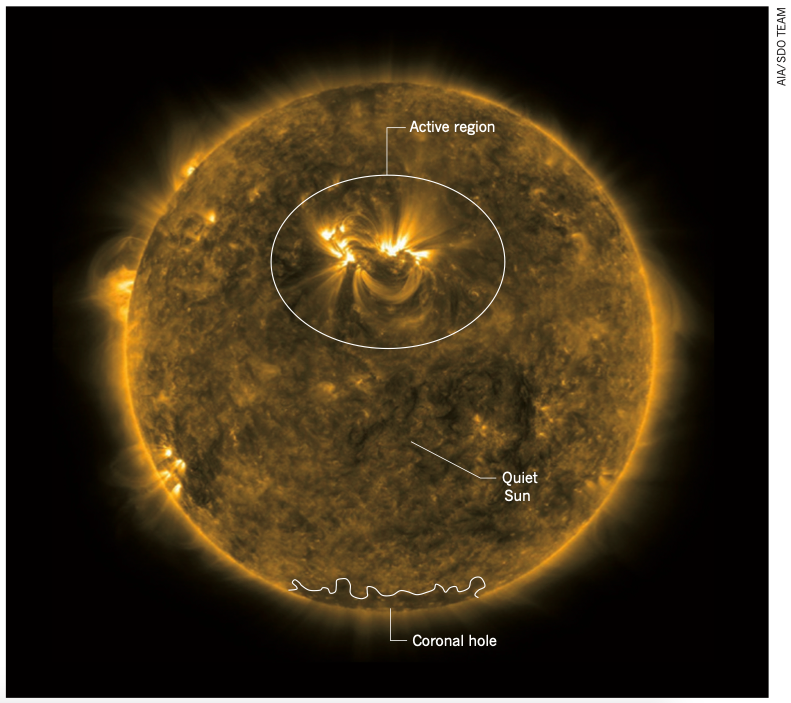
\includegraphics[width=\textwidth]{introduction/active_region_coronal_hole_quiet_sun.png}
    \caption{At a temperature of about 1 million kelvin, this image of coronal plasma was copied from the Atmospheric Imaging Assembly (AIA) instrument on the Solar Dynamics Observatory (SDO). We took the labels from \citet{Cargill2011}. It also offers an example of solar physicists labelling different solar atmosphere parts as either an active region, coronal hole or quiet sun.}
    \label{fig:active_region_quiet_sun_coronal_hole}
\end{figure}

\begin{figure}[!htp]
    \centering
    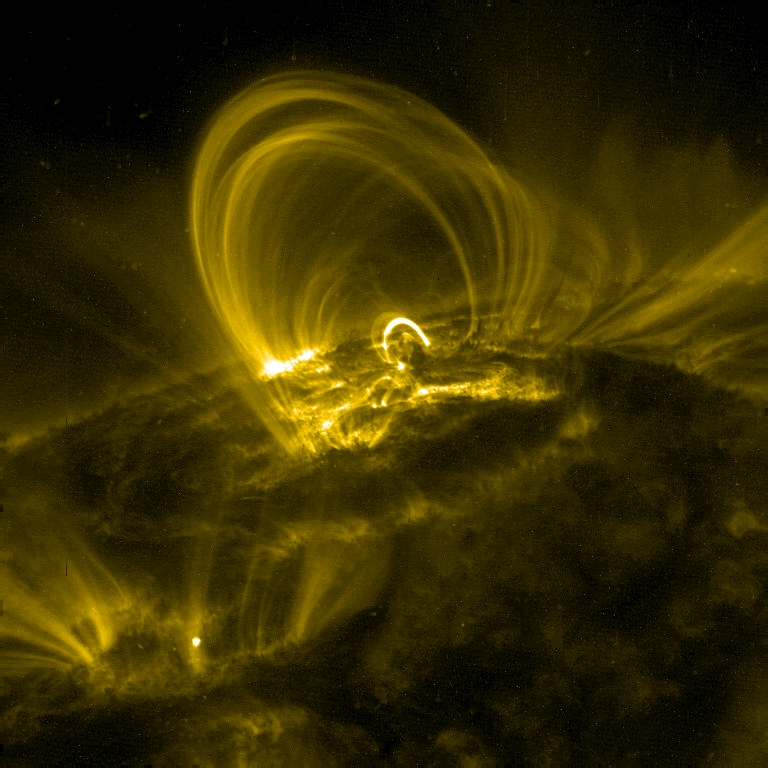
\includegraphics[width=\textwidth]{figures/introduction/coronal_loop_trace.jpg}
    \caption{This image of coronal loops was taken using the TRACE (Transition Region and Coronal Explorer) instrument (courtesy \citet{images_of_coronal_loops}). It shows coronal plasma at a temperature of about 1 million kelvin.}
    \label{fig:coronal_loops_trace}
\end{figure}

\begin{figure}[!htp]
    \centering
    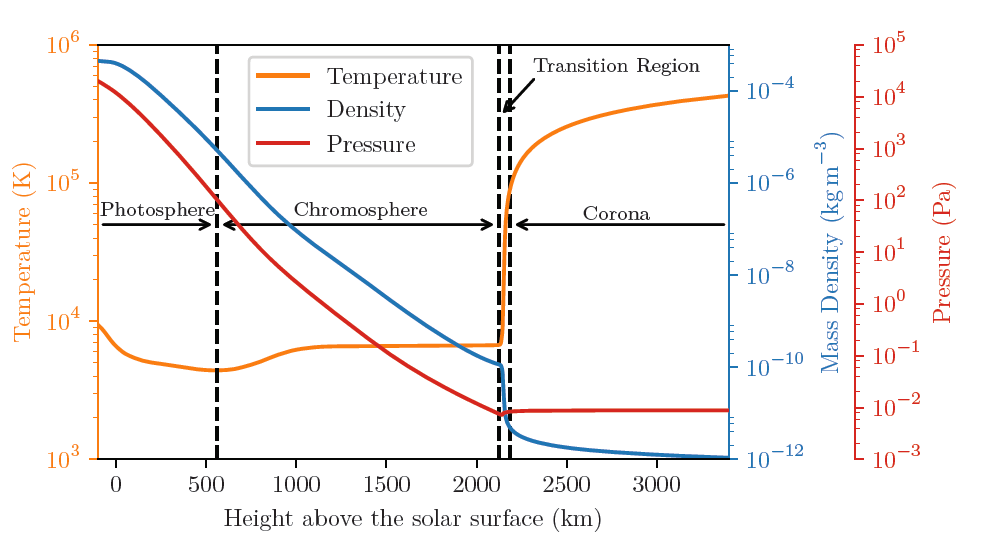
\includegraphics[width=\textwidth]{introduction/VAL.png}
    \caption{The VAL model \citep{Vernazza1981} of the solar atmosphere (courtesy \citet{Williams2018}).}
    \label{fig:VAL_atmosphere}
\end{figure}

\begin{table}[!htp]
    \centering
    \begin{tabular}{c c c c}
        \hline
         & Coronal hole & Quiet Sun & Active region \\
        \hline
        \underline{Corona}  \\
        Conduction & 60 & 200 & $10^3\text{-}10^4$ \\
        Radiation & 10 & 100 & 5000 \\
        Solar wind & 700 & $<50$ & $<100$ \\
        \hline
        Total & 800 & 300 & 10,000 \\
        \hline
        \underline{Chromosphere} \\
        Radiation & 4000 & 4000 & 20,000
        
    \end{tabular}
    \captionof{table}{Order-of-magnitude energy-loss fluxes in $\si{W.m^{-2}}$ \citep{Withbroe1977, Priest2014}.}
    \label{tab:energy_losses_corona_chromosphere}
\end{table}

\begin{figure}[!htp]
    \centering
    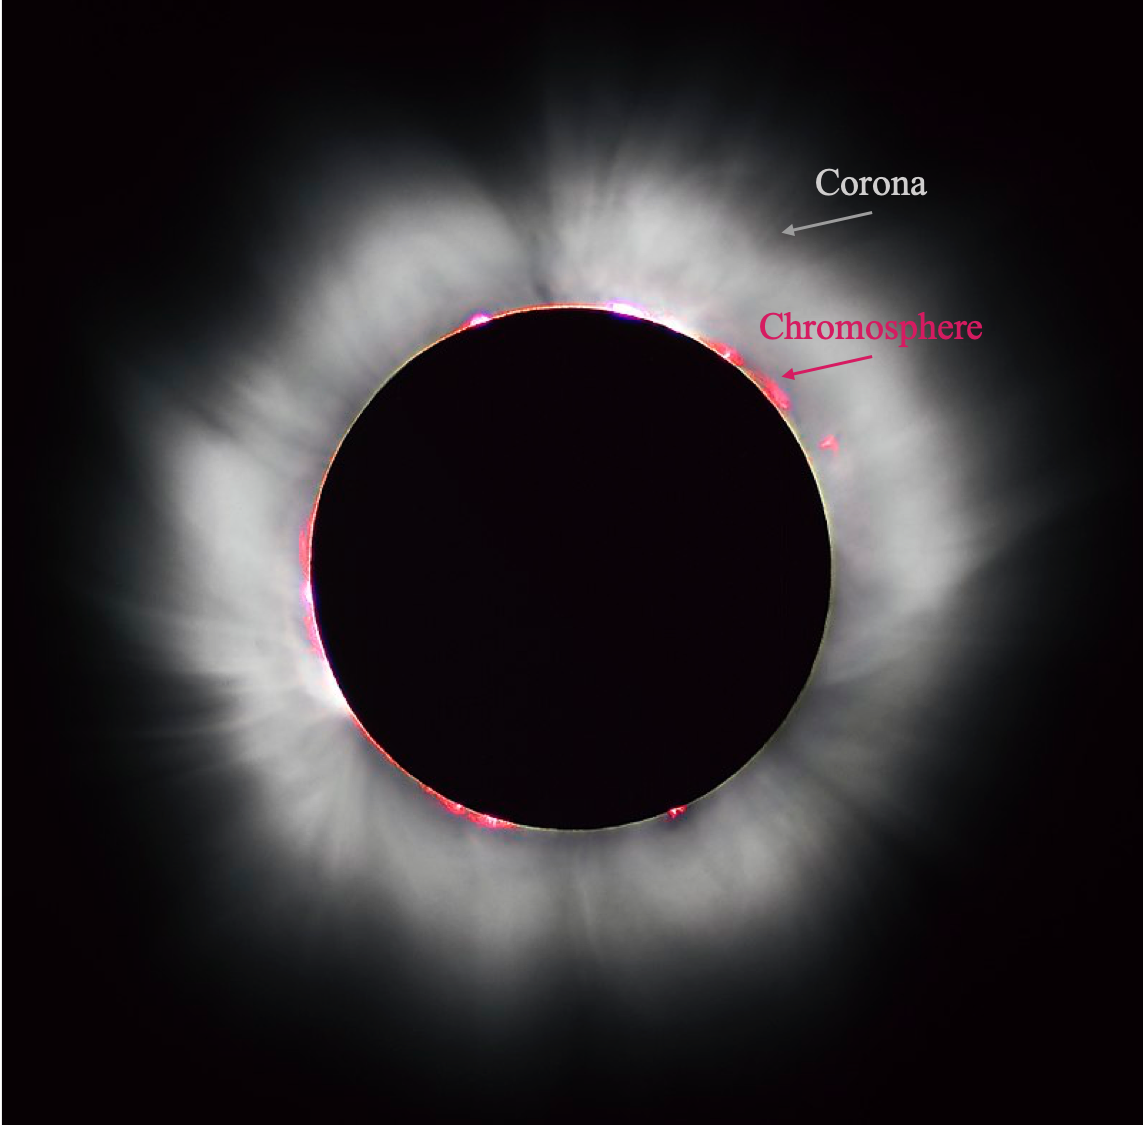
\includegraphics[width=\textwidth]{introduction/eclipse_1999.png}
    \caption{This photo taken in France during the 1999 total eclipse (courtesy Wikimedia, User: Luc Viatour). The chromosphere is emitting a pink/red light close to the disc. The faint white glow around the disk shows white light from the photosphere being Thompson scattered by the corona.}
    \label{fig:total_eclipse1999}
\end{figure}

We label different parts of the solar atmosphere as either an active region, coronal hole or quiet sun (see Figure \ref{fig:active_region_quiet_sun_coronal_hole}). An active region is an area with a strong magnetic field. It is common for sunspots to form in active regions. These are usually the locations where the largest flares and coronal mass ejections occur. Coronal holes are the polar regions of the Sun, which look dark in the X-ray emission. In coronal holes, the magnetic field is usually unipolar and opens towards the interplanetary space. Finally, the quiet Sun usually refers to solar regions that do not lie in either active regions or coronal holes. Note that active regions and the quiet Sun often contain closed loops, like those shown in Figure \ref{fig:coronal_loops_trace}. We refer to these loops as closed because their magnetic field does not extend beyond the solar atmosphere. In contrast, the coronal holes' field lines are referred to as open because they extend far out into the solar system before eventually looping back or connecting with the interplanetary medium.

Figure \ref{fig:VAL_atmosphere} shows data from what is commonly referred to as the Vernazza Avrett and Loeser (VAL) \citep{Vernazza1981} model of the solar atmosphere. It is useful for approximating average values of physical quantities. However, the solar atmosphere is, in reality, a highly inhomogeneous, time-dependent plasma. Figure \ref{fig:VAL_atmosphere} shows that the lowest region is the photosphere. It is the region where most photons, at visible light frequencies, escape into outer space. The chromosphere lies above the photosphere and emits significantly less light than the photosphere. It is only visible with the naked eye during total solar eclipses (see red / pink light in Figure \ref{fig:total_eclipse1999}). The transition region lies between the chromosphere and the corona. Across the transition region, the temperature changes rapidly from approximately $10^5\si{.K}$ to $10^6\si{.K}$. Finally, the corona lies above the chromosphere and transition region. As with the chromosphere, it emits significantly less light than the photosphere and is only visible with the naked eye during total solar eclipses as a white glow (see Figure \ref{fig:total_eclipse1999}). Note that the corona Thompson scatters white light from the photosphere. The intrinsic colour of the corona is not white. However, the chromosphere's inherent colour is indeed the pink/red colour seen in Figure \ref{fig:total_eclipse1999}.

\section{Coronal heating problem}
\label{sec:coronal_heating_problem}

The chromospheric and coronal heating problem relates to the question; `why are they so hot?' It remains one of the biggest unsolved problems in solar physics. Figure \ref{fig:VAL_atmosphere} shows that the temperature increases with distance from the photosphere in the corona and chromosphere. Looking at Figure \ref{fig:VAL_atmosphere}, two questions come to mind. Why does the temperature increase with distance away from the Sun's core? Intuitively, the temperature should decrease away from a heat source. Since the temperature is higher in the corona and chromosphere, this means that conduction is an energy loss mechanism. The plasma is also optically thin in the corona, which means the plasma loses more energy via radiation than it gains. So what is balancing the conductive and radiative losses in the chromosphere and corona?
The energy losses are balanced by converting kinetic and magnetic energy into heat via Ohmic and viscous dissipation \citep{Klimchuk2015}. However, we do not have a verified model giving a precise description of how the temperatures are maintained.

Regarding the first question, we now understand why the solar atmosphere's temperature increases with distance from the Sun's core. For example, \citet{Martens2010} successfully models a similar temperature profile  (although a detailed description of the heating source is still unknown). These models use the internal energy equation with a user-defined heating function superimposed. This heating function simulates the Ohmic and viscous dissipation of magnetic and kinetic energy. They find that even if the heating function is more significant at the footpoints, their models still produce the same basic structure as the solar atmosphere. This counter-intuitive temperature profile is partly explained by the fact that for coronal/chromospheric plasma, the radiative losses can decrease with rising temperature (see for example \citealt{Klimchuck2008}).
However, a detailed description of the primary mechanism(s) by which magnetic and kinetic energy dissipates in the corona has yet to be provided.

In the closed corona, the proposed heating mechanisms can be split into two categories. The first one, relies on the build-up of magnetic energy in the corona which is then suddenly released by magnetic reconnection. The second mechanism brings energy into the corona through MHD waves. In for example \citet{vanBallegooijen2011}, \citet{Howson2020} they model both mechanisms and compare them against each other. Reconnection mechanisms rely on the slow stressing of the magnetic field. We define slow motions as having a period longer than the Alfv\'en travel time of a coronal loop. In Section \ref{sec:case_where_omega=omega_n} we show that if the driving footpoint motions are longer than the Alfv\'en travel time of the loop then this causes the loop to stretch resulting in a large build-up in magnetic energy compared with a small growth in kinetic energy. We show that if the driving motions period is shorter than the Alfv\'en travel time of the loop then the growth in kinetic and magnetic energy is approximately equal. Therefore, for reconnection models, the primary dissipation mechanism is resistive since the amount of free magnetic energy is usually much greater than the amount of free kinetic energy. The amount of free magnetic and kinetic energy associated with the wave is assumed to be approximately equal. Therefore, for wave heating mechanisms the primary dissipation mechanism is usually viscous because the viscous Reynolds number (see Equation \ref{eq:visc_reynolds_number}) is much smaller than the magnetic Reynolds number (see Equation \ref{eq:mag_reynolds_number}).

This thesis will investigate the dissipation of phase mixed Alfv\'en waves and their role in coronal heating. The dissipation of Alfvén waves has been the basis of many coronal heating models (see review by \citealt{Arregui2015} and references therein). Phase mixing was first suggested as a coronal heating mechanism by \citet{Heyvaerts1983}. Phase mixing is the process where gradients perpendicular to the field build-up due to Alfvén waves propagating on field lines with a spatial gradient in Alfvén travel time. This process leads to neighbouring waves moving out of phase with each other; hence the name phase mixing. Other notable mechanisms are: resonant absorption \citep{Ionson1982}, reflection-driven Alfvén wave turbulence \citep{Hollweg1986a,vanBallegooijen2011,Shoda2019}, turbulence triggered via the tearing mode or Kelvin-Helmholtz instability \citep{Browning1984,Antolin2016,Antolin2018} and coupling with compressive modes \citep{Kudoh1999, Antolin2010}.

Table \ref{tab:energy_losses_corona_chromosphere} shows order-of-magnitude estimates for the power-losses (per unit area) in the corona and chromosphere. Note that the mean radiation from the photosphere is significantly greater at about $0.63\times 10^8\si{.W.m^{-2}}$. It is sometimes useful to consider the energy losses per unit volume rather than by per area. The chromosphere’s per unit volume radiative losses can be calculated from the total radiative losses divided by the volume. 
Taking the height difference between the top and bottom of the chromosphere as $1500\si{.km}$ gives the average radiative losses in an active region chromosphere per unit volume as $1.33\times10^{-2}\si{.W.m^{-3}}$. To help get an intuitive idea of how much heat this is, this means that a $1\si{.W}$ light-emitting diode emits about the same radiation as an Olympic sized swimming pool of chromosphere. It is worth noting that the chromosphere and corona are very sparse compared with the photosphere and so a relatively small amount of heat can lead to a large temperature change.
% Taking the height difference between the top and bottom of the chromosphere as $1500\si{.km}$ gives the average radiative losses in the Quiet sun chromosphere per unit volume as $\approx 3\times10^{-3}\si{.W.m^{-3}}$. To put this number in perspective, the average radiative losses from a human is about $100\si{.W}$\footnote{Radiative losses of a human was calculated by using the Stefan-Boltzmann law, where the area of a human was taken to be 2\si{.m^2}, the emissivity of human skin to be unity \citep{emissivity_of_materials}, the temperature of a human as 306\si{.K} and room temperature as 293\si{.K}.}. Therefore, taking the volume of a human as $0.1\si{.m^3}$ gives the radiative losses per volume as $10^3\si{.W.m^{-3}}$. This means that per volume humans emit of the order a million times as much radiation!
% This shows that although the chromosphere and corona have large temperatures they are very sparse and so per volume their radiation is relatively small. 
Note that Table \ref{tab:energy_losses_corona_chromosphere} shows the radiative losses are greater in the chromosphere than in the corona. This is interesting as chromospheric and coronal heating problem is usually referred to as simply the coronal heating problem despite the chromospheric radiative losses being greater.

\section{MHD equations}
\label{sec:mhd equations}

A large fraction of the solar atmosphere is ionised \citep{Shimizu2018} due to the high temperature. The high temperature allows the orbital electrons to break their bonds with their corresponding ions and form free electrons. Therefore, the gas can conduct electricity and is hence a plasma. To study the plasma, we use Magnetohydrodynamics (MHD). The MHD equations are formed by combining equations from electromagnetism with equations from fluid dynamics. Different forms of the MHD equations are used in different contexts. In sections \ref{sec:faradays_law}-\ref{sec:intro_total_energy_eqn} we discuss each of the MHD equations in SI base units.

% \begin{figure}
%     \centering
%     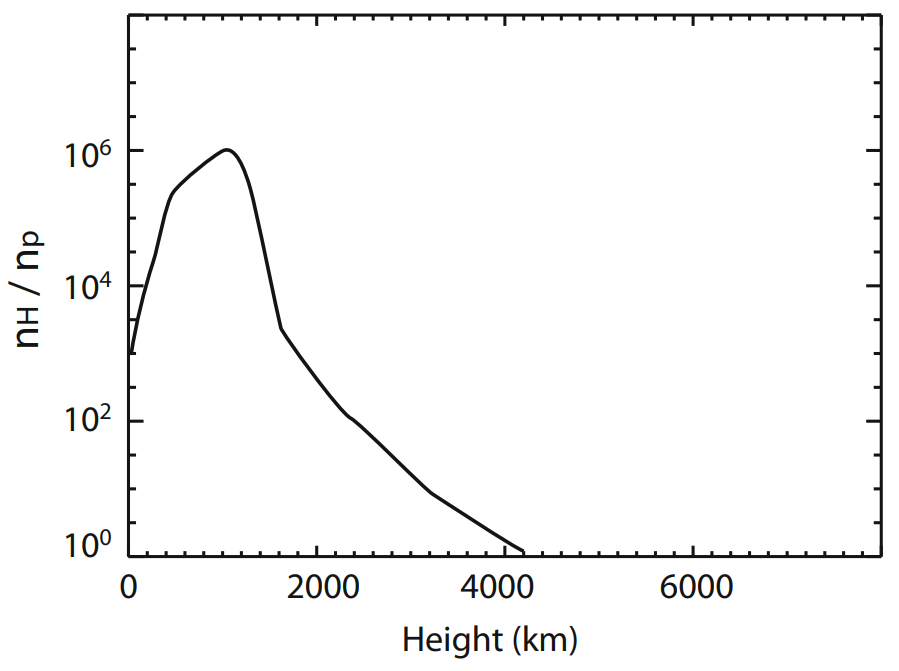
\includegraphics[width=0.5\textwidth]{figures/introduction/partial_ionisation.png}
%     \caption{This figure was taken from \citet{Shimizu2018}. It shows the partial ionisation fraction, $n_H/n_p$, as a function of height in the solar atmosphere, where $n_H$ and $n_p$ denotes the number density of the neutral hydrogen atoms and protons respectively.}
%     \label{fig:partial_ionisation}
% \end{figure}

\subsection{Assumptions}
\label{sec:intro_assumptions}

This thesis is primarily concerned with studying waves in the corona which is assumed to be fully ionised. The Sun's atmosphere is approximately 74\% Hydrogen 25\% Helium and 1\% other elements \citep{sun_vital_statistics}. At typical coronal temperatures, say $10^6\si{.K}$, an electron's thermal energy is approximately $86\si{.eV}$. This is greater than the ionisation energies of Hydrogen and Helium which have first ionisation energies of approximately $14\si{.eV}$ and $25\si{.eV}$ and Helium's second ionisation energy is approximately $54\si{.eV}$ \citep{Lide2003}. Also, the ionisation fraction as a function of height has been estimated in, for example, \citet{Shimizu2018} and suggests that the plasma in the corona is nearly completely ionised. Therefore, in this thesis, we will often model the plasma as fully ionised Hydrogen plasma.

We model the plasma as collisional and assume that collisional transport theory is valid. In \citet{Richardson2019}, they list six conditions for collisional transport theory to be valid. In the strong magnetic field limit, where $\omega_{ce}/\nu_e \gg 1$ (see Table \ref{tab:fundamental_plasma_paramter}) we require
\begin{gather}
    \label{eq:length_scale_condition_parallel}
    L_{||} \gg \lambda_{Te}, \lambda_{Ti}, \\
    \label{eq:length_scale_condition_perpendicular}
    L_\perp \gg \sqrt{\lambda_{Te} r_e}, \sqrt{\lambda_{Ti} r_e}
\end{gather}
where $L_{||}$, $L_\perp$ denote the macroscopic length scales parallel and perpendicular to the magnetic field respectively. In the absence of a magnetic field, we require
\begin{equation}
    \label{eq:length_scale_condition}
    L \gg \lambda_{Te}, \lambda_{Ti},
\end{equation}
where $L$ denotes the macroscopic length scales. For fully ionised Hydrogen plasma, typical values in the corona are,
\begin{gather}
    \begin{aligned}
    \frac{\omega_{ce}}{\nu_e} &= \frac{1}{3.64\times10^{-6}}\frac{eBT^{3/2}}{m_en_e\ln\Lambda} \\
    &\approx 2.42\times10^6\qty(\frac{20}{\ln\Lambda})\qty(\frac{B}{10^{-3}\si{.T}})\qty(\frac{T_e}{10^6\si{.K}})^{3/2}\qty(\frac{10^{15}\si{.m^{-3}}}{n_e}),
    \end{aligned} \\
    \begin{aligned}
    \lambda_{Te} &= \frac{1}{3.64\times10^{-6}}\frac{\sqrt{k_B/m_e}}{\ln\Lambda}\frac{T_e^2}{n_e} \\
    &\approx 0.53\times10^5\qty(\frac{20}{\ln\Lambda})\qty(\frac{T_e}{10^6\si{.K}})^2\qty(\frac{10^{15}\si{.m^{-3}}}{n_e})\si{.m}, 
    \end{aligned} \\
    \begin{aligned}
    \lambda_{Ti} &= \frac{1}{6.00\times10^{-6}}\frac{\sqrt{k_B/m_p}}{\ln\Lambda}\frac{T_i^2}{n_i} \\
    &\approx 0.76\times10^5\qty(\frac{20}{\ln\Lambda})\qty(\frac{T_i}{10^6\si{.K}})^2\qty(\frac{10^{15}\si{.m^{-3}}}{n_i})\si{.m}, 
    \end{aligned} \\
    \begin{aligned}
    r_e & \approx \frac{\sqrt{m_e k_B T_e}}{eB} \\
    &\approx 2.21 \times 10^{-2}\qty(\frac{T_e}{10^6\si{.K}})\qty(\frac{10^{-3}\si{.T}}{B})\si{.m}.
    \end{aligned}
\end{gather}
Therefore, provided the macroscopic length scales are greater than about $1\si{.Mm}$ Equations \eqref{eq:length_scale_condition_parallel}-\eqref{eq:length_scale_condition} should be approximately satisfied.

\begin{table}
    \centering
    {\renewcommand{\arraystretch}{2}% for the vertical padding
        \begin{tabular}{|c|c|c|c|c|}
            \hline
             Name & Symbol & Gaussian units & SI units \\
             \hline
              {\renewcommand{\arraystretch}{0.8}\begin{tabular}[x]{@{}c@{}}Electron\\gyrofrequency\end{tabular}} & $\omega_{ce}$ & $\dfrac{eB}{m_e c}$ & $\dfrac{eB}{m_e}$  \\
             {\renewcommand{\arraystretch}{0.8}\begin{tabular}[x]{@{}c@{}}Ion\\gyrofrequency\end{tabular}} & $\omega_{ci}$ & $\dfrac{ZeB}{m_i c}$ & $\dfrac{ZeB}{m_i}$ \\
             {\renewcommand{\arraystretch}{0.8}\begin{tabular}[x]{@{}c@{}}Electron\\collision rate\end{tabular}} & $\nu_e$ & $2.91\times10^{-6}\dfrac{n_e \ln\Lambda}{T_e^{3/2}}\si{.s^{-1}}$ & $3.64\times10^{-6}\dfrac{n_e \ln\Lambda}{T_e^{3/2}}\si{.s^{-1}}$ \\
             {\renewcommand{\arraystretch}{0.8}\begin{tabular}[x]{@{}c@{}}Ion\\collision rate\end{tabular}} & $\nu_i$ & $4.80\times10^{-8}\dfrac{Z^4n_i \ln\Lambda}{\sqrt{T_i^3m_i/m_p}}\si{.s^{-1}}$ & $6.00\times10^{-8}\dfrac{Z^4n_i \ln\Lambda}{\sqrt{T_i^3m_i/m_p}}\si{.s^{-1}}$ \\
             {\renewcommand{\arraystretch}{0.8}\begin{tabular}[x]{@{}c@{}}Electron\\thermal speed\end{tabular}} & $v_{Te}$ & $\sqrt{\dfrac{k_BT_e}{m_e}}$ & $\sqrt{\dfrac{k_BT_e}{m_e}}$ \\
             {\renewcommand{\arraystretch}{0.8}\begin{tabular}[x]{@{}c@{}}Ion\\thermal speed\end{tabular}} & $v_{Ti}$ & $\sqrt{\dfrac{k_BT_i}{m_i}}$ & $\sqrt{\dfrac{k_BT_i}{m_i}}$ \\
             {\renewcommand{\arraystretch}{0.8}\begin{tabular}[x]{@{}c@{}}Electron\\gyroradius\end{tabular}} & $r_e$ & $\dfrac{v_{Te}}{\omega_{ce}}$ & $\dfrac{v_{Te}}{\omega_{ce}}$ \\
             {\renewcommand{\arraystretch}{0.8}\begin{tabular}[x]{@{}c@{}}Ion\\gyroradius\end{tabular}} & $r_i$ & $\dfrac{v_{Ti}}{\omega_{ci}}$ & $\dfrac{v_{Ti}}{\omega_{ce}}$ \\
             {\renewcommand{\arraystretch}{0.8}\begin{tabular}[x]{@{}c@{}}Electron\\mean free path\end{tabular}} & $\lambda_{Te}$ & $\dfrac{v_{Te}}{\nu_e}$ & $\dfrac{v_{Te}}{\nu_e}$ \\
             {\renewcommand{\arraystretch}{0.8}\begin{tabular}[x]{@{}c@{}}Ion\\mean free path\end{tabular}} & $\lambda_{Ti}$ & $\dfrac{v_{Ti}}{\nu_i}$ & $\dfrac{v_{Ti}}{\nu_i}$ \\
             \hline
        \end{tabular}
    }
    \captionof{table}{This table lists some of the fundamental plasma parameters. The Gaussian formulas were copied from \citet{Richardson2019} which were then converted into SI base units. The collision rates are for completely ionised plasmas. $B$ denotes the magnetic field strength, $e$ denotes the elementary charge, $c$ denotes the speed of light, $m_e$, $m_p$ denote the mass of an electron and proton respectively, $Z$ gives the charge state, i.e. the number of protons in an ion, $n_e$, $n_i$ denote the electron and ion number densities respectively, $\ln \Lambda$ denotes the Coulomb logarithm, $T_e$, $T_i$ denotes the temperature of the electrons and ions respectively and $k_B$ denotes the Boltzmann constant.}
    \label{tab:fundamental_plasma_paramter}
\end{table}

\subsection{Faraday's law}
\label{sec:faradays_law}

Faraday's law is given by
\begin{equation}
    \label{eq:faradays_law}
    \curl\vec{E}=-\pdv{\vec{B}}{t}.
\end{equation}
$\vec{B}$ is the magnetic induction. In solar or astrophysical contexts, it is referred to as the magnetic field strength. In this thesis, $\vec{B}$ will hereafter be referred to as the magnetic field strength. $\vec{E}$ denotes the electric field. Finally, time is denoted with $t$.

\subsection{Amp\`ere's law}
\label{sec:amperes_law}

Amp\`ere's's law is given by
\begin{equation}
    \label{eq:amperes_law}
    \curl{\vec{B}}=\mu_0\vec{j}+\underbrace{\frac{1}{c^2}\pdv{\vec{E}}{t}}_{\approx\,0}
\end{equation}
We approximate the magnetic permeability, $\mu_0$, by its value in a vacuum, namely,
\[\mu_0=4\pi\times10^{-7}\si{.henry.m^{-1}}.\]
The current density is denoted with $\vec{j}$. We approximate the speed of light, $c$, with its value in a vacuum, namely,
\[c=\sqrt{\mu_0\epsilon_0}\approx3.00\times10^8\si{.m.s^{-1}},\]
where $\epsilon_0$ is the permittivity of free space in a vacuum. 

In this thesis, we neglect last term in Equation \eqref{eq:amperes_law}, called the displacement current. Replacing the time derivative with $1/t_0$, and $\vec{E}$ with $E_0$ means that
\[\abs{\frac{1}{c^2}\pdv{\vec{E}}{t}}\approx\frac{1}{c^2}\frac{E_0}{t_0},\]
where $E_0$ and $t_0$ denotes the typical size of their respective quantities. From Faraday's law, Equation \eqref{eq:faradays_law}, it follows that
\[\frac{E_0}{l_0}\approx \frac{B_0}{t_0},\]
where $B_0$ and $l_0$ denote the typical size of their respective quantities. Letting
\[v_0=\frac{l_0}{t_0},\quad \frac{B_0}{l_0}\rightarrow|\curl\vec{B}|,\]
it follows that
\[\abs{\frac{1}{c^2}\pdv{\vec{E}}{t}}\approx\frac{v_0^2}{c^2}\abs{\curl{\vec{B}}},\]
where $v_0$ here denotes a typical speed. Hence, we can neglect the displacement current, provided
\begin{equation}
    \label{eq:v0_less_c}
    v_0\ll c.
\end{equation}
This thesis is interested in waves in the corona. It is very rare for waves to have a velocity amplitude which exceeds the local Alfv\'en speed, $v_A$, given by
\begin{equation}
    v_A\approx\frac{\abs{\vec{B}}}{\sqrt{{\mu}_0\rho}},
\end{equation}
where $\rho$ denotes the plasma density. In the corona, the Alfv\'en speed is approximately $10^6\si{.m.s^{-1}}$ and so condition \eqref{eq:v0_less_c} is satisfied.

% \subsection{Gauss's law}

% Gauss's law is given by
% \begin{equation}
%     \label{eq:gausss_law}
%     \div{\vec{E}}=\underbrace{\frac{\rho^*}{\epsilon_0}}_{\approx\,0},
% \end{equation}
% where $\rho^*$ is the charge density.

\subsection{Solenoidal constraint}

The solenoidal constraint states that
\begin{equation}
    \div{\vec{B}}=0.
\end{equation}
Physically, this equation states that a magnetic field can have no sources or sinks, i.e. no monopoles.

\subsection{Ohm's law}
\label{sec:ohms_law}

\citet{Priest2014} shows that for fully ionised plasma, Ohm's law is given by
\begin{equation}
    \label{eq:ohms_law}
    \vec{E}+\vec{v}\cross\vec{B}=\underbrace{\frac{\vec{j}}{\sigma}}_{\text{Direct / Pedersen term}}+\underbrace{\frac{1}{n_ee}\vec{j}\cross\vec{B}}_{\text{Hall term}},
\end{equation}
where the electron inertia and electron pressure gradient terms have been neglected. We denote the plasma velocity with $\vec{v}$. The Cowling conductivity, $\sigma$, is given by
\begin{equation}
    \sigma = \frac{n_ee^2}{m_e\nu_e}.
\end{equation}
Substituting in typical coronal values, the resistivity coefficients can be approximated by
\begin{gather}
    \frac{1}{\sigma}\approx2.58\times10^{-6}\qty(\frac{T}{10^6\si{.K}})^{-3/2}\si{.mho.m^{-1}},  \\
    \frac{\abs{\vec{B}}}{en_e}\approx6.24\,\qty(\frac{\abs{\vec{B}}}{10^{-3}\si{.T}})\qty(\frac{10^{15}\si{.m^{-3}}}{n_e}).
\end{gather}
The coulomb logarithm, $\ln\Lambda$, lies between 5 and 20 and has a weak temperature dependence. For coronal plasma, a suitable approximation is $\ln\Lambda\approx20$. It is tempting to neglect the direct current term in favour of the Hall term. However, the Hall term is dependent only on currents parallel to the field. Throughout this thesis, the currents perpendicular to the field dominate.

\subsection{Mass continuity}

The mass continuity equation is given by
\begin{equation}
    \label{eq:mass_continuity}
    \pdv{\rho}{t}+\div(\rho\vec{v})=0.
\end{equation}
The mass density is denoted by $\rho$. Physically, this equation states that the rate of mass change in a volume is given by the total flux of mass moving in or out of a fixed volume.

\subsection{Momentum equation}
The most general from of the momentum equation/equation of motion relevant for this thesis is
\begin{equation}
    \label{eq:momentum}
    % \rho\frac{D\vec{v}}{Dt}=\underbrace{\vec{j}\cross\vec{B}}_{\text{Lorentz force}}-\underbrace{\grad p}_{\text{Pressure force}}-\underbrace{\rho g_\odot \vec{\hat{r}}}_{\text{Gravitational force}}+\underbrace{\div\vec{\sigma}_{Brag}}_{\text{Viscous force}}.
    \rho\frac{D\vec{v}}{Dt}=\underbrace{\vec{j}\cross\vec{B}}_{\text{Lorentz force}}-\underbrace{\grad p}_{\text{Pressure force}}-\underbrace{\frac{G\rho}{r^2}\vec{\hat{r}}}_{\text{Gravitational force}}+\underbrace{\div\vec{\sigma}_{Brag}}_{\text{Viscous force}}.
\end{equation}
Here the $D/Dt$ operator denotes the material derivative. The plasma pressure is denoted with $p$.

The first term on the right-hand side of Equation \eqref{eq:momentum} is the Lorentz force. The $\rho^*\vec{E}$ term in the more general form of the Lorentz force has been neglected, where $\rho^*$ denotes the charge density. This is because we model the plasma as electrically neutral. \citet{Priest2014} shows that the plasma can be modelled as electrically neutral provided the length scales of the system, $l_0$, are greater than the Debye length, $\lambda_D$. The Debye length is approximated by
\begin{equation}
    \lambda_D\approx2.18\times10^{-3}\qty(\frac{T}{10^6\si{.K}})^{1/2}\qty(\frac{10^{15}\si{.m^{-3}}}{n})^{1/2}\si{.m}.
\end{equation}
The Lorentz force is commonly split into two components,
\begin{equation}
    \vec{j}\cross\vec{B}=\underbrace{\frac{1}{\mu_0}(\vec{B}\vdot\grad)\vec{B}}_{\text{Magnetic tension force}}\underbrace{-\grad\qty(\frac{B^2}{2\mu_0})}_{\text{Magnetic pressure force}},
\end{equation}
where 
\[\frac{B^2}{2\mu_0}=\frac{\vec{B}\vdot\vec{B}}{2\mu_0},\]
is commonly called the magnetic energy density.

The gravitational force acts radially inward towards the core of the sun, where $\vec{\hat{r}}$ is the unit vector in the radial direction. The gravitational force in the solar atmosphere is approximated by
\begin{equation}
    \label{eq:gravitational_force}
    \frac{G\rho}{r^2}\vec{\hat{r}} = \rho g_\odot \vec{\hat{r}},
\end{equation}
where
\begin{equation}
    \label{eq:gravitational_acceleration}
    g_\odot=\frac{M_\odot G}{R_\odot}\approx274\si{.m.s^{-2}},
\end{equation}
$M_\odot$ denotes the mass of the Sun enclosed by the solar surface, $R_\odot$ is the radius of the solar surface, and $G$ is the gravitational acceleration. Equation \eqref{eq:gravitational_force} is valid in the solar atmosphere provided the height of the plasma above the solar surface, $h$, is less than the solar radius, i.e. $h\ll R_\odot$.

The viscous force is given by the divergence of the Braginskii viscous stress tensor, $\vec{\sigma}_{Brag}$ \citep{Braginskii1965}. Here we present the viscous stress tensor in the same form as in \citet{MacTaggart2017},
\begin{equation}
    \label{eq:braginskii_viscous_stress_tensor}
    \vec{\sigma}_{Brag}=\eta_0\vec{W}^{(0)}+\eta_1\vec{W}^{(1)}+\eta_2\vec{W}^{(2)}
    -(\eta_3\vec{W}^{(3)}+\eta_4\vec{W}^{(4)}),
\end{equation}
where
\begin{gather}
    \vec{W}^{(0)}=\tfrac{3}{2}(\vec{W}\vec{\hat{B}}\cdot\vec{\hat{B}})(\vec{\hat{B}}\otimes\vec{\hat{B}}-\tfrac{1}{3}\vec{I}),\\
    \vec{W}^{(1)}=(\vec{I}-\vec{\hat{B}}\otimes\vec{\hat{B}})\vec{W}(\vec{I}-\vec{\hat{B}}\otimes\vec{\hat{B}})
    +\tfrac{1}{2}(\vec{W}\vec{\hat{B}}\cdot\vec{\hat{B}})(\vec{I}-\vec{\hat{B}}\otimes\vec{\hat{B}}),\\
    \vec{W}^{(2)}=(\vec{I}-\vec{\hat{B}}\otimes\vec{\hat{B}})\vec{W}(\vec{\hat{B}}\otimes\vec{\hat{B}})+(\vec{\hat{B}}\otimes\vec{\hat{B}})\vec{W}(\vec{I}-\vec{\hat{B}}\otimes\vec{\hat{B}}),\\
    \vec{W}^{(3)}=\tfrac{1}{2}\vec{Z}\vec{W}(\vec{I}-\vec{\hat{B}}\otimes\vec{\hat{B}})-\tfrac{1}{2}(\vec{I}-\vec{\hat{B}}\otimes\vec{\hat{B}})\vec{W}\vec{Z}, \\
    \vec{W}^{(4)}=(\vec{Z}\vec{W}\vec{\hat{B}})\otimes\vec{\hat{B}}+\vec{\hat{B}}\otimes(\vec{Z}\vec{W}\vec{\hat{B}}),
\end{gather}
with 
\begin{equation}
    \vec{W}=\vec{\nabla}\vec{v}+(\vec{\nabla}\vec{v})^T-\tfrac{2}{3}(\vec{\nabla}\cdot\vec{v})\vec{I},
\end{equation}
where $\vec{Z}$ is the tensor with components $Z_{ij}=\epsilon_{ikj}b_k$, where $\epsilon_{ikj}$ are components of the Levi-Civita symbol. $\vec{\hat{B}}$ is given by
\begin{equation}
    \vec{\hat{B}}=\frac{\vec{B}}{|\vec{B}|}.
\end{equation}
\citet{Hogan1984} labels each of the tensors, $\eta_0\vec{W}^{(0)}$, $\eta_1\vec{W}^{(1)}$, $\eta_2\vec{W}^{(2)}$, $\eta_3\vec{W}^{(3)}$ and  $\eta_4\vec{W}^{(4)}$ with names based on their physical interpretations. The author labels $\eta_0\vec{W}^{(0)}$ as the viscosity tensor parallel to the magnetic field. $\eta_1\vec{W}^{(1)}$ and $\eta_2\vec{W}^{(2)}$ are labelled as the viscosity tensors perpendicular to the magnetic field. Finally, $\eta_3\vec{W}^{(3)}$ and $\eta_4\vec{W}^{(4)}$ are referred to as the drift contributions. The drift terms are also referred to as the dispersive terms because $\vec{W}^{3}:\grad \vec{v}=\vec{W}^{4}:\grad \vec{v}=0$ which means they do not directly dissipate energy. Note that $\vec{W}^{(0)}$ contains a $\div{\vec{v}}$ term, therefore, it is dependent on derivatives parallel to field field as well as derivatives associated with the compressibility of the velocity. The viscosity coefficients are approximated by
\begin{gather}
    \label{eq:braginskii_eta_0}
    \eta_0=2.21\times10^{-16}\frac{T^{5/2}}{\log \Lambda}\si{.kg.m^{-1}.s^{-1}}, \\
    \label{eq:braginskii_eta_1}
    \eta_1=\frac{3}{10}\eta_0(\omega_{ci}/\nu_i)^{-2}, \\
    \label{eq:braginskii_eta_2}
     \eta_2=4\eta_1,   \\
    \eta_3=\frac{1}{2}\eta_0(\omega_{ci}/\nu_i)^{-1}, \\
    \eta_4=2\eta_3,
\end{gather}
in the strong filed limit ($\omega_{ci}/\nu_i\gg1$). For typical coronal parameters, the product $\omega_{ci}/\nu_i$ for fully ionised hydrogen plasma is approximated by 
\begin{equation}
    \label{eq:proton_gyrofrequency_times_collision_time}
    \begin{aligned}
    \omega_{ci}/\nu_i &= \frac{1}{6.00\times10^{-8}}\frac{eBT_i^{3/2}}{m_in_i\ln\Lambda}\\
    &\approx 0.80\times10^5\qty(\frac{20}{\ln\Lambda})\qty(\frac{B}{10^{-3}\si{.T}})\qty(\frac{T_i}{10^6\si{.K}})^{3/2}\qty(\frac{10^{15}\si{.m^{-3}}}{n_i}).
    \end{aligned}
\end{equation}
Hence, in the corona the condition, $\omega_{ci}/\nu_i\gg1$, is usually satisfied (except near null points). For this reason, authors commonly neglect all of the viscosity tensors except $\vec{W}^{(0)}$ \citep{Hollweg1986b, MacTaggart2017}. However, in this thesis, we find that the gradients perpendicular to the field can be so strong that the $\vec{W}^{(1)}$ tensor cannot be neglected. The Reynolds number associated with $\vec{W}^{(0)}$ is given by
\begin{equation}
    \begin{aligned}
    R_e&=\frac{\rho\abs{\vec{v}\cdot\grad{\vec{v}}}}{\abs{\div{\eta_0\vec{W}^{(0)}}}} \\
    &\approx\frac{\rho_0 l_0V_0}{\eta_0},
    \end{aligned}
\end{equation}
where $\rho_0$ denotes the typical density in the system, $l_0$ denotes the typical length scales of the system and $V_0$ denotes the typical velocity amplitude of the system. According to \citet{McIntosh2011,McIntosh2012}, the velocity amplitude can be approximated as about $10\si{.km.s^{-1}}$. In the corona, we approximate the above Reynolds number as
\begin{equation}
    \label{eq:visc_reynolds_number}
    R_e\approx  0.90\times10^2\qty(\frac{\rho_0}{10^{-12}\si{kg.m^{-3}}})\qty(\frac{l_0}{10^8\si{.m}})\qty(\frac{V_0}{10^4\si{.m.s^{-1}}})\qty(\frac{10^6\si{.K}}{T})^{5/2}.
\end{equation}
Given that the Reynolds number is significantly greater than unity we will often neglect viscosity. Note that if we ignore all viscous and resistive terms, then the equations are ideal.

% Consider the ratio of the Lorentz force with the gravitational force
% \[\frac{|\vec{j}\cross\vec{B}|}{\rho g_\odot}\approx \frac{v_{A0}^2}{v_g^2},\]
% where $v_{A0}$ denotes the typical size of the Alfv\'en speed, and $v_g$ is the gravitational free-fall speed given by
% \begin{equation}
%     v_g = \sqrt{g_\odot l_0},
% \end{equation}
% where $l_0$ gives the characteristic length-scale of the system. In this Thesis we will be studying waves in loops with a maximum length of $100\si{.Mm}$. A typical value for the Alfv\'en speed in the corona is about $1\si{.Mm.s^{-1}}$ \citep{McIntosh2011,McIntosh2012}. Therefore, we can approximate this ratio as
% \begin{equation}
%     \label{eq:ignore_gravity}
%     \frac{v_A^2}{v_g^2}\approx 3.6\times10^1\qty(\frac{v_{A0}^2}{1\si{.Mm^2.s^{-2}}})\qty(\frac{10 \si{.Mm}}{l_0}).
% \end{equation}


% \begin{wrapfigure}{r}{0.5\textwidth}
%   \vspace{-10pt}
%   \begin{center}
%     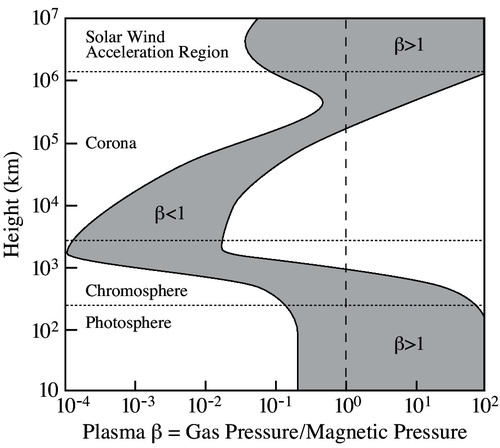
\includegraphics[width = 0.5\textwidth]{figures/introduction/plasma_beta.jpg}
%   \end{center}
%   \vspace{-10pt}
%     % \caption{Courtesy \citet{Gary2001}.}
%      \label{fig:plasma_beta}
% \end{wrapfigure}

Consider the ratio of the pressure force term and Lorentz force term in the momentum equation, Equation \eqref{eq:momentum}, given by
\[\frac{|\grad p|}{|\vec{j}\cross\vec{B}|}\approx \frac{p_0}{B_0^2/\mu}=\frac{\beta}{2},\]
where $p_0$ and $B_0$ denotes the typical size of their respective quantities. The plasma beta, $\beta$, is defined as the ratio of the plasma pressure over the magnetic pressure given by
\begin{equation}
    \label{eq:plasma_beta}
    \beta = \frac{p}{B^2/(2\mu)}.
\end{equation}
Figure \ref{fig:plasma_beta} shows an estimate of the plasma beta as a function of height in the solar atmosphere. It shows that in the solar corona $\beta \ll 1$. Since this Thesis is primarily concerned with modelling waves in the corona, we will often approximate $\beta=0$, which allows us to neglect the pressure force in favour of the Lorentz force.

\begin{figure}
    \centering
    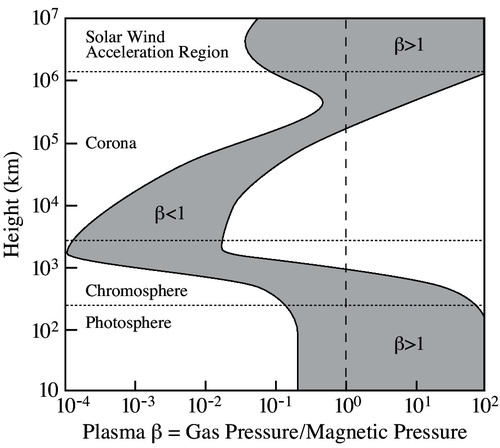
\includegraphics[width = 0.5\textwidth]{figures/introduction/plasma_beta.jpg}
    \caption{The shaded region shows an estimate of the plasma beta in the solar atmosphere as a function of height. This figure was adapted from \citet{Gary2001}.}
    \label{fig:plasma_beta}
\end{figure}

\subsection{Ideal gas law}

For fully ionised Hydrogen plasma the ideal gas law is approximated by
\begin{equation}
    \label{eq:ideal_gas_law}
    p=2\frac{k_B}{m_p}\rho T,
\end{equation}
where $k_B$ denotes the Boltzmann constant approximated by 
\[k_B\approx1.38 \times 10^{-23}\si{.m^2.kg.s^{-2}.K^{-1}}.\]

\subsection{Internal energy equation}
\label{sec:internal_energy_equation}

The most general form of the internal energy equation which we use in this thesis is
\begin{equation}
    \label{eq:internal_energy}
    \pdv{}{t}\qty(\frac{p}{\gamma - 1})+\underbrace{\div(\frac{\gamma p}{\gamma - 1}\vec{v}+\vec{q})}_{\text{Enthalpy flux + Conduction}}=\underbrace{ + \frac{j^2}{\sigma}+\vec{\sigma}_{Brag}:\grad \vec{v}-n^2Q(T)-\vec{v}\vdot\grad{p}}_{\text{Ohmic + Viscous heating $-$ Radiation $-$ Work done}}.
\end{equation}
The internal energy per unit volume is given by $p/(\gamma - 1)$, where $\gamma$ is the ratio of specific heats, also known as the adiabatic index.

The conduction term is given by the divergence of the heat flux vector, $\vec{q}$, where
\begin{equation}
    \vec{q}=-\vec{\kappa}\grad T,
\end{equation}
where $\vec{\kappa}$ is the thermal conduction tensor. The divergence of the heat flux may be split into two parts,
\begin{equation}
    \div\vec{q}=\grad_{||}\vdot(\kappa_{||}\grad_{||}T)+\grad_{\perp}(\kappa_\perp\grad_\perp T),
\end{equation}
where $\grad_{||}$ is given by
\begin{equation}
    \grad_{||}=\vec{\hat{B}}(\vec{\hat{B}}\vdot\grad),
\end{equation}
and $\grad_\perp$ is given by
\begin{equation}
    \grad_\perp = \grad - \grad_{||}.
\end{equation}
The thermal conductivity parallel/perpendicular to the field is denoted with $\kappa_{||}$/$\kappa_\perp$ respectively. In coronal plasma, the conductivity is usually much stronger along the field than it is parallel. The parallel conductivity is approximated by
\begin{equation}
    \kappa_{||}=1.8\times10^{-10}\frac{T^{5/2}}{\ln\Lambda}\si{.W.m^{-1}.K^{-1}},
\end{equation}
and the ratio $\kappa_\perp/\kappa_{||}$, for typical coronal parameters, is approximated by
\begin{equation}
    \frac{\kappa_\perp}{\kappa_{||}}=2\times10^{-13}\qty(\frac{n}{10^{15}\si{.m^{-3}}})^2\qty(\frac{10^6\si{.K}}{T})^3\qty(\frac{10^{-3}\si{.T}}{B})^2
\end{equation}
(in the strong field limit, where $\omega_{ci}/\nu_i\gg1$, see \citealt{Spitzer1965, Braginskii1965, Priest2014}). In the corona, the parallel conductivity dominates (except near null points), so we usually neglect the perpendicular conduction.

$Q(T)$ denotes the optically thin radiative loss function. See for example \citet{Rosner1978, Klimchuck2008, Dere2009, Priest2014} for details on the radiative loss function in the solar corona. 
% According to \citet{Klimchuck2008} the radiative loss function, $Q(T)$, is  approximated by (with units $\si{W.m^{3}}$)
% \begin{equation}
% \label{eq:radiative_loss_function}
% Q(T)=\begin{cases}
%     1.09\times10^{-44}T^2, & \text{for } T\le10^{4.97}, \\
%     8.87\times10^{-30}T^{-1}, & \text{for } 10^{4.97}<T\le10^{5.67}, \\
%     1.90\times10^{-35}, & \text{for } 10^{5.67}<T\le10^{6.18}, \\
%     3.53 \times 10^{-26}T^{-3/2}, & \text{for } 10^{6.18}<T\le10^{6.55}, \\
%     3.46 \times 10^{-38}T^{1/3}, & \text{for } 10^{6.55}<T\le10^{6.90}, \\
%     5.49 \times 10^{-29} T^{-1}, & \text{for } 10^{6.90}<T\le10^{7.93}, \\
%     1.96\times 10^{-40} T^{1/2}, & \text{for } 10^{7.93}<T.
% \end{cases}
% \end{equation}
% Note that \citet{Klimchuck2008} gives the radiative losses in units of $\si{erg.s^{-1}.cm^{3}}$ so a conversion factor of $10^{13}$ was used to convert the units into SI base units.
\citet{Klimchuk2015} (and references therein) shows that the temperature evolution of coronal loops is dependent on the time interval, $\Delta t$, between nanoflares/heating events. If the timescale between nanoflares is significantly shorter than the cooling timescale of a loop through conduction and radiation, i.e. $\Delta t \ll \tau_{cool}$, then the temperature evolution can be approximately isothermal (see the left-side of Figure \ref{fig:klimchuck_temperature}). However, if the heating concentrates near the loop footpoints then a loop may be in a state of thermal non-equilibrium, see e.g. \citet{Antiochos2000, Johnston2019}. If the time interval between nanoflares is significantly longer than the cooling timescale, i.e. $\Delta t \gg \tau_{cool}$, then a loop can change in temperature significantly (see the right-side of Figure \ref{fig:klimchuck_temperature}). For simplicity, in this thesis, we will model the plasma as isothermal.

\begin{figure}
    \centering
    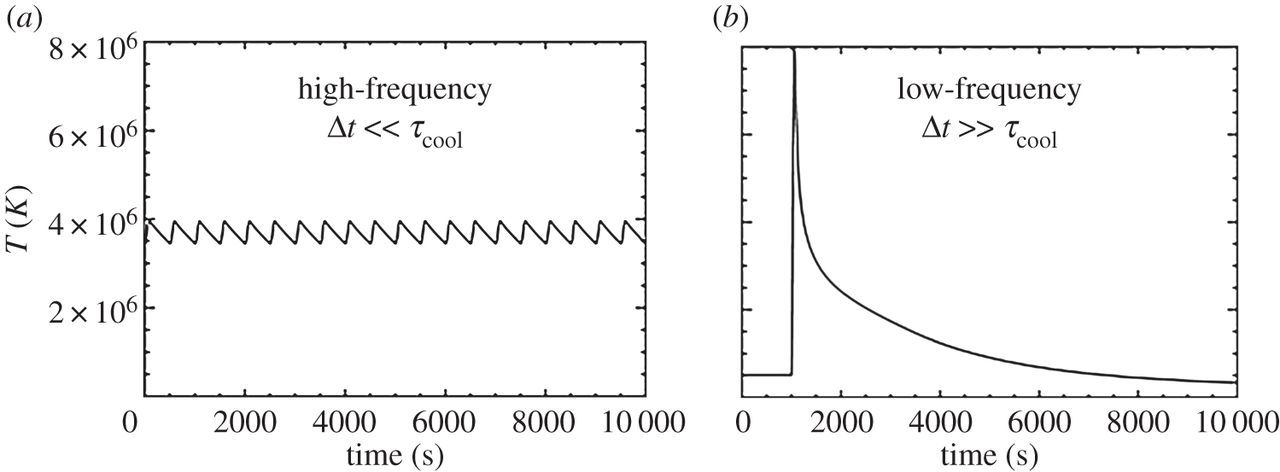
\includegraphics[width=\textwidth]{figures/introduction/klimchuck_temperature.jpg}
    \vspace{-20pt}
    \caption{This figure was copied from \citet{Klimchuk2015}. It shows the temperature evolution in a coronal loop heated by high frequency nanoflares (left) and low-frequency nanoflares (right).}
    \label{fig:klimchuck_temperature}
\end{figure}

% Throughout most of this thesis we model the thermodynamics as adiabatic. In other words, we approximate the internal energy equation as
% \begin{equation}
%     \pdv{}{t}\qty(\frac{p}{\gamma - 1})+\div(\frac{\gamma p}{\gamma - 1}\vec{v})=0.
% \end{equation}
% The Ohmic and viscous heating can be neglected, provided their respective Reynolds numbers satisfy $R_e\gg1$ and $R_m\gg1$ (see Equations \eqref{eq:visc_reynolds_number} and \eqref{eq:mag_reynolds_number}). This thesis is mainly concerned with the evolution of waves. We can neglect conduction and radiation provided the conductive and radiative timescales are much longer than that of a wave period. The timescale at which the pressure changes due to radiation, $\tau_r$, can be approximated by
% \begin{equation}
%     \frac{1}{\gamma - 1}\frac{p_0}{\tau_r}\approx n_0^2Q(T_0),
% \end{equation}
% where $p_0$ denotes the typical pressure in the system $n_0$ denotes the typical number density and $T_0$ denotes the typical temperature. In coronal conditions, with a temperature of $T=10^6\si{.K}$ and an adiabatic index of $\gamma=5/3$, $\tau_r$ can be approximated by
% \begin{equation}
%     \tau_r\approx 0.79\times10^{3}\qty(\frac{p_0}{10^{-2}\si{.Pa}})\qty(\frac{10^{15}}{n_0})^2\si{.s}.
% \end{equation}
% Estimating the conductive timescale is more difficult because it requires knowledge of the temperature length scales which changes by at least an order of magnitude from the corona to the transition region. We can make use of the results from \citet{Withbroe1977} (see Table \ref{tab:energy_loss_fluxes}) to see that the conductive losses are approximately double that of the radiative losses. Hence, in the corona, the timescale of conductive losses, $\tau_c$, is approximately given by
% \begin{equation}
%     \tau_c\approx3.95\times10^2\si{.s}.
% \end{equation}
% These results tell us that conduction and radiation can be neglected for waves with a frequency much greater $10^{-2}\si{.Hz}$.
% A typical coronal loop has a length of say $50\si{.Mm}$ and an Alfv\'en speed of $1\si{.Mm.s^{-1}}$, this gives a fundamental time period of $100\si{s}$. \textcolor{red}{Talk about the Morton power spectrum here, to show the frequencies in which we can ignore. Make your own data and graphs by using the formulas in Paolo's paper. To be honest we can't justify ignoring conduction and radiation. But linear waves do little to affect the density and pressure, so we could simulate it by making our background Alfv\'en speed a function of time.}
% \begin{equation}
%     \frac{1}{\gamma - 1}\frac{p_0}{\tau_c}\approx\frac{\kappa_{||}T_0}{l_0^2},
% \end{equation}
% where $p_0$ denotes the typical pressure in the system, $T_0$ denotes a typical temperature and $l_0$ denotes a typical length-scale for the temperature variations. Hence
% \begin{equation}
%     \tau_c\approx\qty(\frac{p_0}{10^{-2}\si{.Pa}})\qty(\frac{l_0}{10^6\si{.m}})^2\qty(\frac{10^6\si{.K}}{T_0})^{7/2}
% \end{equation}

\subsection{Induction equation}
\label{sec:induction_eqn}

Faraday's law, Equation \eqref{eq:faradays_law}, can be combined with Ohm's law, Equation \eqref{eq:ohms_law}, to give the induction equation,
\begin{equation}
    \label{eq:induction_equation}
    \pdv{\vec{B}}{t}=\underbrace{\curl(\vec{v}\cross\vec{B})}_{\text{Ideal term}}-\underbrace{\curl(\frac{\vec{j}}{\sigma}+\frac{1}{n_ee}\vec{j}\cross\vec{B})}_{\text{Non-ideal term}}.
\end{equation}
In Section \ref{sec:ohms_law}, we showed that if $B_0 / (n_e e) \ll \sigma^{-1}$ or $\vec{j_{||}\gg\vec{j}_\perp}$ then we can neglect the Hall term. Additionally, if we assume that the spatial derivatives of $\sigma$ can be neglected then by using Amp\`ere's law, Equation \eqref{eq:amperes_law} (the induction equation), be written as
\begin{equation}
    \pdv{\vec{B}}{t}=\underbrace{\curl(\vec{v}\cross\vec{B})}_{\text{Advective term}}+\underbrace{\eta\laplacian\vec{B}}_{\text{Diffusive term}},
\end{equation}
where $\eta$ is the magnetic diffusivity, given by
\begin{equation}
    \label{eq:eta_typical_values}
    \begin{aligned}
        \eta&=\frac{1}{\mu_0\sigma} \\
        &\approx 2.06\qty(\frac{T}{10^6\si{.K}})^{-3/2}\si{.m^2.s^{-1}},
    \end{aligned}
\end{equation}
for typical coronal temperatures. The magnetic Reynolds number is defined as
\begin{equation}
    R_m=\frac{l_0V_0}{\eta}\sim\frac{\text{Advective term}}{\text{Diffusive term}},
\end{equation}
where $l_0$ denotes the system's typical length scales and $V_0$ denotes the typical velocity in the system. In the corona, the magnetic Reynolds number can be approximated by
\begin{equation}
    \label{eq:mag_reynolds_number}
    R_m\approx4.86\times10^{9}\qty(\frac{l_0}{10^6\si{.m}})\qty(\frac{V_0}{10^4\si{.m.s^{-1}}})\qty(\frac{T_0}{10^6\si{.K}})^{3/2}.
\end{equation}
We usually neglect the diffusive term in the induction equation in favour of the advective term. However, sometimes the length scales can become sufficiently small that we cannot ignore the diffusion term. Note that our approximation for the corona's velocities uses results from \citet{McIntosh2011,McIntosh2012}.

For typical values, $R_m$, given by Equation \eqref{eq:mag_reynolds_number}, is approximately 8 orders of magnitude larger than $R_e$, given by Equation \eqref{eq:visc_reynolds_number}. This suggests viscous dissipation dominates over resistive. However, this order of magnitude analysis does not consider the fact that gradients perpendicular to the field may be orders of magnitude greater than gradients parallel to the magnetic field. Moreover, there could be significantly more free magnetic energy to dissipate compared with kinetic energy. Note that \citet{vanDoorsselaere2007} uses observations to suggest that resistive heating dominates over viscous.

\subsection{Total energy equation}
\label{sec:intro_total_energy_eqn}

Taking the dot product of Equation \eqref{eq:momentum} with $\vec{v}$ gives
\[\rho\pdv{}{t}\qty(\frac{v^2}{2}) + \rho\vec{v}\cdot\grad(\frac{1}{2}v^2)=\vec{v}\cdot\grad{p} + \vec{v}\cdot(\vec{j}\cross\vec{B}) - \vec{v}\cdot(\rho\grad{\Phi})+\vec{v}\cdot\div{\vec{\sigma}_{Brag}},\]
where $\rho\Phi=\rho g_{\odot}r$ gives the gravitational potential energy density (assuming the gravitational force is given by Equation \ref{eq:gravitational_force}). We can simplify this by using the following identity 
\[\div(\vec{\sigma}_{Brag}\vec{v})=\vec{v}\cdot\div{\vec{\sigma}_{Brag}^T} + \vec{\sigma}_{Brag}:\vec{v},\]
from Equation (1.11.16) of \citet{Kelly2020}, where $\vec{\sigma}_{Brag}:\vec{v}=\tr(\vec{\sigma}_{Brag}\grad{\vec{v}})$ denotes the double-dot product. Note that $\vec{\sigma}_{Brag}$ is symmetric, i.e. $\vec{\sigma}_{Brag}=\vec{\sigma}_{Brag}^T$.
Multiplying Equation \eqref{eq:mass_continuity} with $v^2/2$ gives
\[\frac{v^2}{2}\pdv{\rho}{t}+\frac{v^2}{2}\div(\rho\vec{v})=0.\]
The time-derivative of the gravitational potential energy density gives
\[\pdv{\rho\Phi}{t}=-\Phi\div{\rho\vec{v}}.\]
Combining the above equations gives the equation for the kinetic and gravitational energy,
\[
    \pdv{}{t}\qty(\frac{1}{2}\rho v^2 + \rho\Phi) + \div\qty(\frac{1}{2}\rho v^2\vec{v}+\rho\Phi\vec{v} - \vec{\sigma}_{Brag}\vec{v})=-\vec{v}\cdot\grad{p}+\vec{v}\cdot(\vec{j}\cross\vec{B})-\vec{\sigma}_{Brag}:\vec{v}.
\]

Taking the dot product of Equation \eqref{eq:faradays_law} with $\vec{B}/\mu$ gives
\[\begin{aligned}
\pdv{}{t}\qty(\frac{B^2}{2\mu})&=-\frac{\vec{B}}{\mu}\cdot\curl{\vec{E}} \\
&=-\div(\frac{\vec{E}\cross\vec{B}}{\mu})-\vec{E}\cdot\vec{j}.
\end{aligned}\]
Substituting Equation \eqref{eq:ohms_law} gives the equations for the magnetic energy density,
\[
    \pdv{}{t}\qty(\frac{B^2}{2\mu})+\div(\frac{\vec{E}\cross\vec{B}}{\mu})=-\vec{v}\vdot(\vec{j}\cross\vec{B})-\frac{j^2}{\sigma}.
\]

Therefore the rate of change of total energy is given by
\begin{equation}
    \pdv{}{t}\qty(\frac{1}{2}\rho v^2 + \frac{B^2}{2\mu}+\frac{p}{\gamma-1}+\rho\Phi)+\div{\vec{S}}=-n^2Q(T),
\end{equation}
where
\begin{equation}
    \vec{S} = \frac{1}{2}\rho v^2\vec{v} + \frac{\vec{E}\cross\vec{B}}{\mu} + \frac{\gamma p}{\gamma - 1}\vec{v} + \vec{q} + \rho\Phi\vec{v} - \vec{\sigma}_{Brag}\vec{v}.
\end{equation}

% \section{Our model of a coronal loop}

% This thesis is primarily concerned with the dynamics of waves in coronal loops, like the ones pictured in Figure \ref{fig:coronal_loops_trace}. Throughout this thesis, we study waves by considering perturbations on a background equilibrium. The goal of this section is to provide an overview of our simplest background equilibrium. Our background equilibrium is designed to be as simple as possible, for mathematical convenience, while being complex enough to simulate in a meaningful manner the dynamics of waves in coronal loops. In this section, we aim to clearly show the simplifications which have been made and discuss the likely consequences of these simplifications. We denote background variables with a subscript 0. Later on, in Section \ref{sec:mhd_waves_dispersion_relation}, we will label our perturbed quantities with a subscript 1. Where the time derivatives of the equilibrium quantities are zero.

% Throughout most of this thesis, including this introductory chapter, we model the loops as straight. \textcolor{red}{In chapter X, we look at waves in non-straight magnetic fields}. In other words our background magnetic field, $\vec{B}_0$ given by 
% \begin{equation}
%     \vec{B}_0=B_0\vec{\hat{z}},
% \end{equation}
%, where $B_0$ is a constant and $z$, gives the coordinate along the field. In general, the coronal field is curved, however, the concepts outlined here can still be applied. The effects of loop curvature on coronal kink oscillations are investigated in \citet{vanDoorsselaere2009}. 

% We model our equilibrium as static i.e. $\vec{v}_0=0$ and adiabatic i.e. the internal energy equation is approximated as,
% \begin{equation}
%     \pdv{}{t}\qty(\frac{p}{\gamma - 1})+\div(\frac{\gamma p}{\gamma - 1}\vec{v})=0.
% \end{equation}
% Since the velocity is static and the background field is potential the Ohmic and viscous heating are zero.


% From the mass continuity, Equation \eqref{eq:mass_continuity}, we can see that a static velocity implies that the equilibrium density, $\rho_0$, does not change with time. Moreover, from the induction equation, Equation \eqref{eq:induction_equation}, we can see that the background magnetic field, $\vec{B}_0$, does not change with time. The momentum equation, \eqref{eq:momentum}, shows that for the velocity to remain static, we require
% \begin{equation}
%     \vec{j}_0\cross\vec{B}_0-\grad p_0 - \rho_0 g_\odot\vec{\hat{r}}=0.
% \end{equation}
% Our background field is uniform, therefore, $\vec{j}_0=\vec{0}$. We model the pressure as being in hydrostatic balance, i.e. we assume that
% \begin{equation}
%     \grad p_0 = 
% \end{equation}

% We model the loops as being in thermal equilibrium, i.e. we assume the internal energy does not change with time. This is done for mathematical convenience. See, for example, \citet{Antiochos2000, Johnston2019} for more information on the thermal non-equilibrium in coronal loops. We model the equilibrium temperature and density as not changing with time, therefore, the pressure, $p_0$, does not change with time. Since conduction and radiation are both energy loss mechanisms in the corona, there must be some heating term balancing these losses to maintain thermal equilibrium. We label this coronal heating term $H_c$. Plugging in our equilibrium values into the internal energy equation, Equation \eqref{eq:internal_energy}, with the coronal heating term included, gives
% \begin{equation}
%     \pdv{}{z}\qty(\kappa_{||}\pdv{T_0}{z})+n^2Q(T)=H_c
% \end{equation}

% The coordinate along the loop is $z$. We model the gravity as though the loop were a semi-circle. The gravitational force, $\vec{F}_g$, is given by
% \begin{equation}
%     \vec{F}_g=\sin(\frac{\pi z}{L})g_{\odot}\rho\vec{\hat{z}}.
% \end{equation}
% We assume the loop is in hydrostatic balance.

% Below are listed some of the key assumptions that we make. A diagram of our loop is illustrated in Figure X.
% \begin{enumerate}
%     \item Throughout most of this thesis, including this introductory chapter, we model the loops as straight. \textcolor{red}{In chapter X, we look at waves in non-straight magnetic fields}. In general, the coronal field is curved, however, the concepts outlined here can still be applied. We model the gravity as though the loop were a semi-circle. The gravitational force, $\vec{F}_g$, is given by
%     \begin{equation}
%         \vec{F}_g=\sin(\frac{\pi z}{L})g_{\odot}\rho\vec{\hat{z}}
%     \end{equation}
%     \item We approximate the transition region as a discontinuity. This means that we model the temperature, density and pressure as being discontinuous at the transition region.  When studying waves, the transition region can be approximated as a discontinuity provided the wavelength of the wave is longer than the width of the transition region.
%     \item We model the temperature in the corona as isothermal. In reality, the temperature of a typical coronal loop increases with height. We model our equilibrium as being in hydrostatic balance and so by assuming isothermal temperature this means we are overestimating the scale height of the density.
% \end{enumerate}

\section{MHD waves: Dispersion relation}
\label{sec:mhd_waves_dispersion_relation}

Solving the MHD equations is notoriously difficult. Some of the basic properties of the Navier-Stokes equations, which is a subset of the MHD equations, are not known. There is a famous problem known as the Navier–Stokes existence and smoothness problem. The Clay Mathematics Institute in May 2000 made this problem one of its seven Millennium Prize problems in mathematics. It offered a \$1,000,000 prize to the first person to solve the problem. The challenge is to prove or give a counter-example of the following statement:
\begin{displayquote}
In three space dimensions and time, given an initial velocity field, there exists a vector velocity and a scalar pressure field, which are both smooth and globally defined, that solve the Navier–Stokes equations.
\end{displayquote}

Due to the difficulty in solving the MHD equations, solutions are usually calculated numerically. To obtain an analytic solution, we study a simplified plasma. Analytical solutions are useful as a starting point for understanding plasma dynamics. Moreover, parameters can be arbitrary constants which allows a large parameter space to be studied simultaneously. Typically, numerical simulations only calculate the solution for a single set of parameters, and then the simulation has to be restarted for different parameter values.

Given that the corona has a large Reynolds number (see Equations \ref{eq:visc_reynolds_number} and \ref{eq:mag_reynolds_number}) we model the plasma as ideal. Additionally, the plasma beta in the corona is small (see Figure \ref{fig:plasma_beta}) so we assume the only force in the momentum equation is the Lorentz force. This gives the momentum equation as
\begin{equation}
    \label{eq:momentum_eqn_beta=0}
    \rho\frac{D \vec{v}}{D t}=\frac{1}{\mu}(\curl{\vec{B}})\cross\vec{B},
\end{equation}
the induction equation as
\begin{equation}
    \label{eq:induction_eqn_ideal}
    \pdv{\vec{B}}{t}=\curl(\vec{v}\cross\vec{B}),
\end{equation}
and mass continuity equation as,
\begin{equation}
    \tag{\ref{eq:mass_continuity}}
    \pdv{\rho}{t}+\div(\rho\vec{v})=0.
\end{equation}
% Finally, we model the plasma as isothermal, see Section \ref{sec:internal_energy_equation},
% \begin{equation}
%     T = T_0(\vec{x}),
% \end{equation}
% note that the pressure can be calculated from the ideal gas law, Equation \eqref{eq:ideal_gas_law}.

We model small perturbations on a static background equilibrium in other words we assume
\begin{gather}
    \label{eq:linear_assumotion_v}
    \vec{v}(\vec{x},t) = \vec{u}(\vec{x},t),\ \text{where}\ u\ll v_A,\\
    \label{eq:linear_assumotion_b}
    \vec{B}(\vec{x},t) = \vec{B}_0(\vec{x}) + \vec{b}(\vec{x},t),\ \text{where}\ b\ll B_0, \\
    \label{eq:linear_assumotion_rho}
    \rho(\vec{x},t) = \rho_0(\vec{x}) + \rho_1(\vec{x},t),\ \text{where}\ \rho_1\ll \rho_0,
\end{gather}
where
\[u = \abs{\vec{v}},\ B_0=\abs{\vec{B}_0}\ ,b=\abs{\vec{b}}.\] Note that $\vec{B}_0$ and $\rho_0$ are referred to as the background quantities which are specified beforehand and $\vec{v}$, $\vec{b}$ and $\rho_1$ are the perturbed quantities which need to be calculated.
We assume $u\ll v_A$ because observations suggest $u / v_A$ to be approximately in the range [$10^{-2}$,\ $10^{-1}$] \citep{McIntosh2011,McIntosh2012}. We approximate $\pdv*{\vec{B}_0}{t}=0$ since magnetic structures can last much longer than the typical frequency and Alfv\'en travel time of waves in a coronal loop. If we take the Alfv\'en speed in the corona as about $1\si{.Mm.s^{-1}}$ \citep{McIntosh2011} and assume that coronal loops have a characteristic length of about 100$\si{.Mm}$ \citep{O'Neill2005} then This gives an Alfv\'en travel time of about $100\si{.s}$. Magnetic structures can last much longer than this, for example, active region prominences can last a few hours or a day, while quiescent prominences can last between a few and 300 days \citep{Priest2014}. We assume that $\pdv*{\rho_0}{t}$ and this approximately holds in coronal loops which are isothermal. \citet{Klimchuk2015} shows that loops can be approximated as isothermal if the time interval between heating events/nanoflares in the loops is sufficiently small..
% We will see in \textcolor{red}{Equation X} that provided
% \[f\gg \frac{\langle v_A \rangle}{L},\]
% then
% \[\frac{b}{\sqrt{\mu}}\sim \sqrt{\rho}u,\]
% where $f$ denotes the frequency of the wave, $\langle v_A \rangle$ denotes the average Alfv\'en speed along the length of a loop and $L$ denotes the length of the loop. Hence, if $u\ll v_A$ then this implies that $b\ll B_0$. \textcolor{red}{Note that typical values for L vA and f are THIS and we typically study waves with frequencies greater than.} Note that if 
% \[f\ll \frac{\langle v_A \rangle}{L},\]
% then it is possible for
% \[\frac{b}{\sqrt{\mu}}\gg \sqrt{\rho}u.\]
% We justify, in part, the assumption given by Equation \eqref{eq:linear_assumotion_rho} by modelling the plasma as isothermal. Therefore, provided the background pressure, $p_0$, remains constant, then by the ideal gas law, Equation \eqref{eq:ideal_gas_law}, the background density, $\rho_0$, must also remain constant is perhaps the hardest to justify. In Section \ref{sec:internal_energy_equation} we showed that conduction and radiation can lead to changes in the plasma pressure and density in a timescale, $\tau_c$, which is comparable to that of typical wave frequencies we will be studying. Moreover, research has shown that loops are typically in a state of thermal nonequilibrium and this can lead to the density growing or shrinking by a factor greater than 2 over a timescale $\tau_c$ \citep{Antiochos2000, Johnston2020}. However, modelling the background density, $\rho_0$ as static is a useful place to start to build our intuition. Future research will look at waves in a domain where the background density evolves with time.

The final assumption we make, in this section, is to assume the background quantities are uniform, primarily because this allows the equations to be solved analytically more easily. Without loss of generality, we can model the background magnetic field as being directed in the $z$-direction, i.e.
\begin{equation}
    \label{eq:background_field}
    \vec{B}_0=B_0\vec{\hat{z}}.
\end{equation}
With these assumptions in place we can simplify Equation \eqref{eq:momentum_eqn_beta=0} and \eqref{eq:induction_eqn_ideal} via a linearization procedure. This is where we neglect terms involving the product of small terms i.e. $\vec{u}$, $\vec{b}$ or $\rho_1$ and neglect the time-derivatives of the background terms $\vec{B}_0$, $\rho_0$. The momentum equation reduces to
\begin{equation}
    \label{eq:momentum_eqn_linear}
    \begin{aligned}
        \pdv{\vec{u}}{t}&=\frac{1}{\mu\rho_0}(\curl{\vec{b}})\cross\vec{B}_0 \\
        &=\frac{B_0}{\mu\rho_0}\qty[(\vec{B}_0\cdot\grad)\vec{b} - \grad\qty(\frac{\vec{b}\cdot\vec{B}_0}{2\mu})].
    \end{aligned}
\end{equation}
The induction equation simplifies to
\begin{equation}
    \begin{aligned}
    \pdv{\vec{b}}{t}&=\curl(\vec{u}\cross\vec{B}_0) \\
    &=(\vec{B}_0\cdot\grad)\vec{u} - \vec{B}_0\div{\vec{u}},
    \end{aligned}
\end{equation}
and the mass continuity equation is given by
\begin{equation}
    \pdv{\rho_1}{t}+\div(\rho_0\vec{v})=0.
\end{equation}
Note that $\vec{u}$ and $\vec{b}$ are independent of $\rho_1$ and so we only need to solve for $\vec{u}$ and $\vec{b}$.
Written out component-wise the above equations become
\begin{gather}
    \pdv{u_x}{t} = v_{A0}^2\qty[\pdv{\hat{b}_x}{z} - \pdv{\hat{b}_z}{x}],\\
    \label{eq:uy_eqn_linear}
    \pdv{u_y}{t} = v_{A0}^2\qty[\pdv{\hat{b}_y}{z} - \pdv{\hat{b}_z}{y}],\\
    \label{eq:bx_eqn_linear}
    \pdv{\hat{b}_x}{t} = \pdv{u_x}{z},\\
    \label{eq:by_eqn_linear}
    \pdv{\hat{b}_y}{t} = \pdv{u_y}{z},\\
    \pdv{\hat{b}_z}{t} = -\qty[\pdv{u_x}{x} + \pdv{u_y}{y}],
\end{gather}
where
\begin{gather}
    \label{eq:b_hat}
    \vec{\hat{b}}=\frac{\vec{b}}{B_0}=(\hat{b}_x,\hat{b}_y,\hat{b}_z),\\
    v_{A0} = \frac{B_0}{\sqrt{\mu\rho_0}}.
\end{gather}
Since the Lorentz force is perpendicular to the background field, $u_z$, is decoupled and can be treated separately. We can eliminate $\hat{b}_x$ and $\hat{b}_y$ from the above equations to give
\begin{gather}
    \label{eq:ux_in_terms_of_bz}
   \qty(\pdv[2]{}{t}-v_{A0}^2\pdv[2]{}{z})u_x=-v_{A0}^2\pdv{\hat{b}_z}{x}{t}, \\
    \label{eq:uy_in_terms_of_bz}
   \qty(\pdv[2]{}{t}-v_{A0}^2\pdv[2]{}{z})u_y=-v_{A0}^2\pdv{\hat{b}_z}{y}{t}.
\end{gather}
Eliminating $\hat{b}_z$ gives
\begin{gather}
   \qty[\pdv[2]{}{t}-v_{A0}^2\qty(\pdv[2]{}{x}+\pdv[2]{}{z})]u_x=v_{A0}^2\pdv{u_y}{x}{y}, \\
    \label{eq:uy_in_terms_of_ux}
   \qty[\pdv[2]{}{t}-v_{A0}^2\qty(\pdv[2]{y}+\pdv[2]{}{z})]u_y=v_{A0}^2\pdv{u_x}{x}{y}.
\end{gather}
Eliminating $u_y$ gives
\[\qty[\pdv[2]{}{t}-v_{A0}^2\qty(\pdv[2]{y}+\pdv[2]{}{z})]\qty[\pdv[2]{}{t}-v_{A0}^2\qty(\pdv[2]{}{x}+\pdv[2]{}{z})]u_x=v_{A0}^4\frac{\partial^4 u_x}{\partial x^2 \partial y^2},\]
\[\begin{aligned}
\implies &\qty[\pdv[2]{}{t}-v_{A0}^2\pdv[2]{}{z}]\qty[\pdv[2]{}{t}-v_{A0}^2\qty(\pdv[2]{}{x}+\pdv[2]{}{z})]u_x=\\
&v_{A0}^2\pdv[2]{}{y}\qty{v_{A0}^2\pdv[2]{}{x}+\qty[\pdv[2]{}{t}-v_{A0}^2\qty(\pdv[2]{}{x}+\pdv[2]{}{z})]}u_x,
\end{aligned}\]
hence
\begin{equation}
    \implies \qty[\pdv[2]{}{t}-v_{A0}^2\pdv[2]{}{z}]\qty[\pdv[2]{}{t}-v_{A0}^2\qty(\pdv[2]{}{x}+\pdv[2]{}{y}+\pdv[2]{}{z})]u_x=0.
\end{equation}
Since all the coefficients are constant, we can use Fourier analysis to calculate an analytic solution which satisfies the above equation. We assume $u_x$ is of the form
\[u_x = u_{x0}\exp[i(k_x x + k_y y + k_z z + \omega_n t)],\]
where $k_x$, $k_y$, $k_z$ and $\omega_n$ $\in \mathds{C}$.
This reduces our PDE to the following algebraic equation
\begin{equation}
    [\omega_n^2 - v_{A0}^2k_z^2][\omega_n^2 - v_{A0}^2(k_x^2+k_y^2+k_z^2)] = 0.
\end{equation}
The above dispersion equation shows that four types of solution can exist. The solutions are given by
\[\omega_1 = v_{A0}k_z,\]
\[\omega_2 = -v_{A0}k_z,\]
\[\omega_3 = v_{A0}\sqrt{k_x^2 + k_y^2 + k_z^2},\]
\[\omega_4 = -v_{A0}\sqrt{k_x^2 + k_y^2 + k_z^2}.\]
Solutions where $\omega = \omega_1$ or $\omega_2$ are called Alfv\'en wave solutions and solutions where $\omega = \omega_3$ or $\omega_4$ are fast wave solutions. The next two subsections go into further detail about each wave, respectively.

For now, we calculate the solution for the case where the perturbed quantities, $u_x$, $u_y$, $\hat{b}_x$, $\hat{b}_y$ and $\hat{b}_z$ have an $x$, $y$, $z$ and $t$ dependence of the form
\[f(x,y,z,t)=f_0\exp[i(k_xx + k_y y + k_z z + \omega_n t)],\]
where
\[\omega = \pm v_{A0}k_z.\]
Let $u_{x0}$ be fixed, from Equation \eqref{eq:uy_in_terms_of_ux} we know that
\begin{equation}
    \label{eq:uy0}
    u_{y0} = \frac{v_{A0}^2 k_x k_y}{\omega^2 - v_{A0}^2(k_y^2 + k_z^2)}u_{x0}.
\end{equation}
From Equations \eqref{eq:bx_eqn_linear} and \eqref{eq:by_eqn_linear} we know that
\begin{gather}
    \label{eq:bx0}
    \hat{b}_{x0} = \frac{k_z}{\omega}u_{x0}, \\
    \label{eq:by0}
    \hat{b}_{y0} = \frac{k_z}{\omega}u_{y0}.
\end{gather}
From Equation \eqref{eq:ux_in_terms_of_bz} we know that
\begin{equation}
    \label{eq:bz0}
    \hat{b}_z = -\frac{\omega^2 - v_{A0}^2k_z^2}{k_x \omega} u_{x0}.
\end{equation}

\subsection{Alfv\'en waves}

We define Alfv\'en waves \citep{Alfven1942} as waves with a velocity amplitude, $\vec{u}$, which satisfy the Alfv\'en wave equation, which is given by
\begin{equation}
    \label{eq:alfven_wave_equation}
    \mathcal{L}\vec{u} = \qty(\pdv[2]{}{t} - \frac{1}{\mu\rho}(\vec{B}_0\cdot\grad)^2)\vec{u}=0,
\end{equation}
where $\mathcal{L}$ denotes the Alfv\'en wave equation operator and $\vec{B}_0$ denotes the background magnetic field. This shows that Alfv\'en waves propagate parallel to the background magnetic field with speed given by the Alf\'en speed. Note that for our configuration above the Alfv\'en wave equation operator, $\mathcal{L}$, becomes
\begin{equation}
    \label{eq:alfven_wave_equation_operator}
    \mathcal{L} = \pdv[2]{}{t} - v_{A0}\pdv[2]{}{z}.
\end{equation}
Equations \eqref{eq:ux_in_terms_of_bz} and \eqref{eq:uy_in_terms_of_bz} show that if $\mathcal{L}u_x=\mathcal{L}u_y=0$ then $b_z=b_z(z)$. Therefore, applying the initial condition that $b_z$ is initially zero ensures $b_z=0$ $\forall t$. Note that $b_z$ gives the perturbation in magnetic pressure. For this reason, Alfv\'en waves can be thought of as kinetic-tension waves as they are an oscillation in kinetic and magnetic tension energy. Very much like waves on a guitar string but with magnetic tension replaced with tension in the string.

% A useful quantity is the Poynting flux, $\vec{S}$ given by
% \begin{equation}
%     \label{eq:poynting_flux}
%     \begin{aligned}
%     \vec{S}&=\frac{\vec{E}\times\vec{b}}{\mu} \\
%     & = \frac{1}{\mu}\qty[(\vec{B}_0\cdot\vec{b})\vec{u}-(\vec{u}\cdot\vec{b})\vec{B}_0].
%     \end{aligned}
% \end{equation}
% where $\vec{E}$ denotes the electric field and we approximate it by linearizing Ohm's law (Equation \eqref{eq:ohms_law}) and assuming ideal MHD to give
% \begin{equation}
%     \vec{E}=-\vec{u}\times\vec{B}_0.
% \end{equation}
% This gives the directional energy flux, to see this consider the following.
% Taking the dot product of Equation \eqref{eq:momentum_eqn_linear} with $\rho_0 \vec{u}$ gives
% \[\pdv{}{t}\left(\frac{1}{2}\rho_0 u^2\right)=\frac{1}{\mu}\vec{u}\cdot\qty[(\vec{B}_0\cdot\vec{\nabla})\vec{b}-\vec{\nabla}(\vec{B}_0\cdot\vec{b})].\]
% Taking the dot product of Equation \eqref{eq:induction_eqn_ideal} with $\vec{b}$ gives
% \[\pdv{}{t}\left(\frac{b^2}{2\mu}\right)=\frac{1}{\mu}\vec{b}\cdot\qty[(\vec{B}_0\cdot\vec{\nabla})\vec{u}-\vec{B}_0(\div\vec{u})].\]
% Note that
% \[\pdv{}{t}\qty(\frac{1}{2}\rho_0 u^2 + \frac{b^2}{2\mu})=-\frac{1}{\mu}\div\qty[(\vec{B}_0\cdot\vec{b})\vec{u} - (\vec{u}\cdot\vec{b})\vec{B}_0],\]
% Hence, the energy equation is given by
% \begin{equation}
%     \pdv{}{t}\qty(\frac{1}{2}\rho u^2+\frac{b^2}{2\mu}) + \div{\vec{S}}=0.
% \end{equation}
% This confirms that $\vec{S}$ does indeed give the energy flux for the magnetic and kinetic energy. For Alfv\'en waves, the magnetic pressure perturbation is zero, therefore, the Poytning flux is directed along the magnetic field (see Equation \eqref{eq:poynting_flux}). This means that Alfv\'en waves can only propagate parallel to the magnetic field.

Note that if $\omega=\pm k_z v_A$ then Equations \eqref{eq:uy0}-\eqref{eq:bz0} simplify to
\begin{gather}
    \label{eq:uy0_alfven}
    u_{y0} = -\frac{k_x}{k_y}u_{x0}, \\
    \hat{b}_{x0} = \pm \frac{u_{x0}}{v_{A0}}, \\
    \hat{b}_{y0} = \pm \frac{u_{y0}}{v_{A0}}, \\
    \hat{b}_{z0} = 0.
\end{gather}
This shows that the magnetic pressure perturbation is zero and so all the energy is contained within the magnetic tension.

It is also worth noting that our Alfv\'en wave is invariant in the  $\vec{u}$-direction, in other words,
\begin{equation}
\begin{aligned}
    \div{\vec{u}} &= i(u_xk_x  + u_yk_y) \\
    &= 0\ \text{(using Equation \ref{eq:uy0_alfven}).}
\end{aligned}
\end{equation}
This means the Alfv\'en wave is incompressible.

\subsection{Fast waves}

We define fast waves in $\beta=0$ plasma as waves with velocity amplitude, $\vec{u}$, which satisfy the classical wave equation,
\begin{equation}
    \qty(\pdv[2]{}{t}+v_A^2\laplacian)\vec{u}=0.
\end{equation}
This shows that fast waves propagate isotropically with a speed given by the Alfv\'en speed.
Note that this is only valid for $\beta=0$ plasma, for $\beta\ll 1$ then the fast wave propagates perpendicular to the field at a speed of approximately $v_A + c_s$ and parallel to the field at a speed of $v_A$, where $c_s$ gives the background sound speed. For a derivation of the dispersion relation of fast waves (and its sibling slow waves) in a $\beta>0$ plasma, see for example \citet{Priest2014, Roberts2019}.
 

Note that if $\omega=\pm v_{A0}\sqrt{k_x^2 + k_y^2 + k_z^2}$, then Equations \eqref{eq:uy0}-\eqref{eq:bz0} simplify to
\begin{gather}
    \label{eq:uy0_fast}
    u_{y0}=\frac{k_y}{k_x}u_{x0}, \\
    \label{eq:bx0_fast}
    \hat{b}_{x0} = \pm\frac{k_z}{\sqrt{k_x^2 + k_y^2 + k_z^2}}\frac{u_{x0}}{v_{A0}}, \\
    \label{eq:by0_fast}
    \hat{b}_{y0} = \pm\frac{k_z}{\sqrt{k_x^2 + k_y^2 + k_z^2}}\frac{u_{y0}}{v_{A0}}, \\
    \label{eq:bz0_fast}
    \hat{b}_{z0} = \mp\frac{k_x^2+k_y^2}{k_x\sqrt{k_x^2 + k_y^2 + k_z^2}}\frac{u_{x0}}{v_{A0}},
\end{gather}
The above equation shows that, unlike Alfv\'en waves, the magnetic pressure perturbation, $b_z$, is in general non-zero. Fast waves are oscillations in kinetic and magnetic energy, where the restoring force can be magnetic tension and the magnetic pressure. More generally, in a $\beta>0$ plasma, the plasma pressure also acts as a restoring force and contributes towards the energy associated with the fast wave.

The fast wave is compressible, however, it is invariant in the $\vec{\hat{B}}_0\cross\vec{u}$, direction, in other words,
\begin{equation}
\begin{aligned}
    (\vec{\hat{z}}\cross \vec{u})\vdot\grad &= (-u_y \vec{\hat{x}} + u_x \vec{\hat{y}})\vdot\grad \\
    &= i(-u_yk_x + u_xk_y) \\
    &= 0\ \text{(using Equation \eqref{eq:uy0_fast}).}
\end{aligned}
\end{equation}
In the last section we showed that the Alfv\'en waves are invariant in the $\vec{u}$ direction. Therefore, there is always at least one invariant direction for both our fast and Alfv\'en waves.

\subsection{Poynting flux}

The Poynting flux, $\vec{S}$ is given by
\begin{equation}
    \label{eq:poynting_flux_linear}
    \begin{aligned}
    \vec{S}&=\frac{\vec{E}\times\vec{b}}{\mu} \\
    & = \frac{1}{\mu}\qty[(\vec{B}_0\cdot\vec{b})\vec{u}-(\vec{u}\cdot\vec{b})\vec{B}_0].
    \end{aligned}
\end{equation}
where $\vec{E}$ denotes the electric field and we approximate it by linearizing Ohm's law (Equation \eqref{eq:ohms_law}) and assuming ideal MHD to give
\begin{equation}
    \label{eq:ideal_linear_ohms_law}
    \vec{E}=-\vec{u}\times\vec{B}_0.
\end{equation}
$\vec{S}$ gives the directional energy flux, to see this consider the following.
Taking the dot product of Equation \eqref{eq:momentum_eqn_linear} with $\rho_0 \vec{u}$ gives
\[\pdv{}{t}\left(\frac{1}{2}\rho_0 u^2\right)=\frac{1}{\mu}\vec{u}\cdot\qty[(\vec{B}_0\cdot\vec{\nabla})\vec{b}-\vec{\nabla}(\vec{B}_0\cdot\vec{b})].\]
Taking the dot product of Equation \eqref{eq:induction_eqn_ideal} with $\vec{b}$ gives
\[\pdv{}{t}\left(\frac{b^2}{2\mu}\right)=\frac{1}{\mu}\vec{b}\cdot\qty[(\vec{B}_0\cdot\vec{\nabla})\vec{u}-\vec{B}_0(\div\vec{u})].\]
Note that
\[\pdv{}{t}\qty(\frac{1}{2}\rho_0 u^2 + \frac{b^2}{2\mu})=-\frac{1}{\mu}\div\qty[(\vec{B}_0\cdot\vec{b})\vec{u} - (\vec{u}\cdot\vec{b})\vec{B}_0],\]
Hence, the energy equation is given by
\begin{equation}
    \label{eq:total_energy_eqn_linear}
    \pdv{}{t}\qty(\frac{1}{2}\rho u^2+\frac{b^2}{2\mu}) + \div{\vec{S}}=0.
\end{equation}
This confirms that $\vec{S}$ does indeed give the energy flux for the magnetic and kinetic energy. For Alfv\'en waves, the magnetic pressure perturbation is zero. Therefore, the Poynting flux points along the magnetic field (see Equation \eqref{eq:poynting_flux_linear}).


\section{MHD waves: power spectrum}
\label{sec:mhd_waves_power_spectrum}

MHD waves are ubiquitous and have been observed in for example \citet{Tomczyk2007,McIntosh2011,DeMoortel2012}. These observations are useful for constraining theoretical models and may help answer unsolved problems such as the coronal heating problem. Measurements of the waves' amplitude and wavelength could play an important role in deciding whether MHD waves play an essential or negligible role in coronal heating. Note that the Ohmic and viscous heat provided by MHD waves typically increases with larger wave amplitudes and shorter wavelengths.  A power spectrum can represent the wave amplitude and frequency. This section aims to give a brief overview of the power spectrum of velocity fluctuations in the corona and explain how we calculate it.

In for example \citet{Morton2016,Morton2019}, the power spectrum of velocity fluctuations in the solar corona is calculated. They produce a time sequence, $\{v_n\}$, of the Doppler velocities on the limb of the corona using data from the Coronal Multi-channel Polarimeter (CoMP). CoMP only has a finite cadence and they can only observe the fluctuations for a finite time. Therefore, the observed velocities, $\{v_n\}$, can only be measured at a finite discrete sequence of times $\{t_n\}$. If $N$ measurements are made, i.e.
\[\{v_n\}=v_0, v_1, ... v_{N-1},\]
then we can write 
\[\begin{aligned}
v_n &= \frac{1}{N}\sum_{k=0}^{N-1}V_k\exp(2i\pi  k n / N) \\
&= \frac{1}{N}\sum_{k=0}^{N-1}V_k\exp(2i\pi f_k t_n),
\end{aligned}\]
where
\[t_n = n\Delta t,\]
\[f_k = \frac{k}{N \Delta t},\]
and $\{V_k\}$ is the discrete Fourier transform of $\{v_n\}$, given by
\[\begin{aligned}
V_k&=\sum_{n=0}^{N-1}v_n\exp(-2i\pi k n / N) \\
&=\sum_{n=0}^{N-1}v_n\exp(-2i\pi f_k t_n).
\end{aligned}\]
Note that a measure of the average energy associated with the velocity fluctuations is given by
\begin{equation}
    \langle v^2 \rangle = \frac{1}{N}\sum_{n=0}^{N-1}v_n^2.
\end{equation}
By the Plancheral theorem
\begin{equation}
    \langle v^2 \rangle = \frac{1}{N^2}\sum_{k=0}^{N-1}|V_k|^2.
\end{equation}
Therefore, $|V_k|^2/N^2$ gives a useful measure of the average energy associated with each frequency, $f_k$, for the signal, $\{v_n\}$. Note that $|V_k|$ is Hermitian-symmetric because $\{v_n\}$ is strictly real, i.e.
\begin{equation}
    V_k = \bar{V}_{N-k},\quad \text{for}\ 1 \le k\le N-1,
\end{equation}
% where
% \begin{equation}
%     N_{mid} = \begin{cases}
%     N / 2 - 1, & \text{for}\ N\ \text{even}, \\
%     (N - 1) / 2, & \text{for}\ N\ \text{odd},
%     \end{cases}
% \end{equation}
where $\bar{V}_{N-k}$ denotes the complex conjugate and $\lfloor\,\rfloor$ denotes the floor function which rounds down to the nearest integer. Therefore, we define the power spectrum, $P_k[\{v_n\}]$, as
\begin{equation}
    \label{eq:discrete_power_spectrum_definition}
    P_k[\{v_n\}] = \frac{1}{N^2}\begin{cases}
    |V_0|^2, & \text{for}\ k=0,\\
    |V_k|^2, & \text{for}\ k=N/2\ \text{and}\ N\ \text{even},\\
    2|V_k|^2, & \text{otherwise},\\
    \end{cases}
\end{equation}
where $k=0,1...,\lfloor N / 2\rfloor$. This ensures that $P_k[\{v_n\}]$ satisfies
\begin{equation}
    \langle v^2 \rangle = \sum_{k=0}^{\lfloor N / 2 \rfloor}P_k[\{v_n\}].
\end{equation}

\begin{figure}
    \vspace{-20pt}
    \centering
    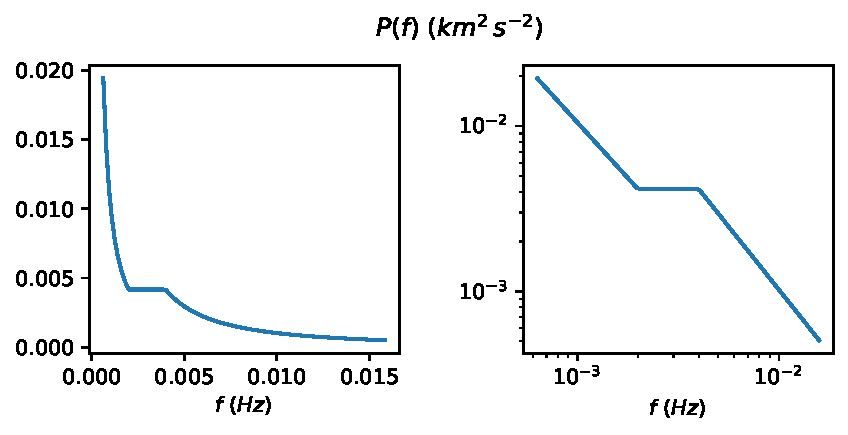
\includegraphics[width=\textwidth]{figures/introduction/power_spectrum_morton.pdf}
    \vspace{-35pt}
    \caption{This figure shows the approximate power spectrum for velocity fluctuations in the corona using data from \citet{Morton2016} and an approximation used in \citet{Pagano2019}. The left-hand side uses a linear axis while the right-hand side uses a log-log axis. The code used to make this figure is available on GitHub in the following directory:\newline
    \href{https://github.com/aleksyprok/apkp_thesis/blob/main/Python/Introduction/power_spectrum.py}{$\rightarrow$ Python/Introduction/power\_spectrum.py}}
    \vspace{-10pt}
    \label{fig:power_spectrum_morton}
\end{figure}

To plot the average power spectrum, $P(f)=P_k[\{v_n\}]$, we will use an approximation given in \citet{Pagano2019} which uses data from \citet{Morton2016}. They state that the power spectrum in $\si{km^2.s^{-2}}$ can be approximated as
\begin{equation}
    P(f) = \begin{cases}
    10^{-6}f^{-1.34},     & 10^{-3.2} \le f \le 10^{-2.7}, \\
    10^{-2.38},           & 10^{-2.7} \le f \le 10^{-2.4}, \\
    10^{-6.05}f^{-1.53}, & 10^{-2.4} \le f \le 10^{-1.8}, \\
    \end{cases}
\end{equation}
where the frequency is measured in $\si{Hz}$. 
Note that the dimensions of $P(f)$ are somewhat meaningless without knowledge of the number of points used, however, for now, we are only interested in the shape of the power spectrum. \cite{McIntosh2011,McIntosh2012}  measured the average amplitude of velocity fluctuations in the corona. They show that observed amplitudes are of the order 10$\si{.km.s^{-1}}$. $P(f)$ is plotted in Figure \ref{fig:power_spectrum_morton}. We can only plot the power spectrum for a finite range of frequencies because the equipment’s cadence is limited. Moreover, we can only observe features for about half a solar rotation before moving out of view. Here the frequency range is $10^{-3.2}\si{.Hz} \le f \le 10^{-1.8}\si{.Hz}$. \citet{Podesta2007} is able to observe higher frequency waves in the solar wind.

\section{Outline of the thesis}

This thesis aims to improve our understanding of MHD waves' dynamics in the solar atmosphere by using models which are complex enough to build our intuition and simple enough to easily be comprehended. In Chapter \ref{chap:ideal_footpoint_driven_alfven_waves} we study the simplest type of MHD wave, namely, Alfv\'en waves. These are waves with a velocity amplitude which satisfies the Alfv\'en wave equation (Equation \ref{eq:alfven_wave_equation}). Our goal is to introduce some of the key concepts relevant to the rest of the thesis. We calculate the solutions for the case where we impose a footpoint driver as a boundary condition. We aim to calculate the solution for when the driver is sinusoidal and a white/red noise force. After that, we extend the model by allowing waves to leak out of the corona.

In Chapter \ref{chap:resistive_phase_mixed_alfven_waves} our goal is to assess the viability of a process called phase mixing as a heating mechanism. We study linear Alfv\'en waves with resistivity and viscosity included in the model with the $y$-direction assumed invariant. We show that if neighbouring field lines have different natural frequencies, this can lead to the formation of steep gradients across the field via phase mixing. To test if this is a viable heating mechanism, we introduce a quantity called the heating rate per unit of wave energy which we denote with $\gamma$. We estimate the required heating rate by assuming it must balance our estimates of the corona's conductive and radiative losses. We also use observational data of velocity fluctuations to estimate the average wave energy in the corona. Using these values, we calculate that $\gamma$ needs to equal about $10^{-1}\si{.s^{-1}}$ for a wave heating mechanism to play a major role in coronal heating. We calculate a theoretical upper bound for $\gamma$ and use this to test if the dissipation of phase-mixed Alfv\'en wave is a viable heating mechanism. Our model also includes partial reflection and allows for a power spectrum of harmonics to be excited.

Chapter \ref{chap:resonant_absorption_in_an_oblique_field} allows for $\pdv*{}{y}\ne0$. This enables a phenomenon called resonant absorption to occur. This is where a propagating fast wave with a given frequency gets absorbed by a magnetic field line, called the resonant field line, with the same natural Alfv\'en frequency. Energy concentrates at the resonant field line and the waves form a standing Alfv\'en wave. We model the magnetic field to be at an arbitrary angle, $\alpha$, to the transition region. In for example, \citet{Halberstadt1993,Halberstadt1995,Arregui2003}, they show that in general, steep boundary layers / evanescent fast waves form. However, their model only includes the corona, and they impose line-tied boundary conditions. This chapter includes the chromosphere and corona and tests if the boundary layers still form if we do not impose line-tied boundary conditions. This allows us to test if the boundary layers are physical or fictitious artefacts generated by using line-tied boundary conditions.

Finally, in Chapter \ref{chap:conclusions_and_future_work} a summary of results from each of the chapters is given, and we discuss ideas for further study.